%!TEX program = xelatex
%% Copyright (C) 2025 傅祉珏
%% 
%% 此文件是《全景图拼接实验报告》的LaTeX源码,依据AGPLv3许可证发布。
%% 完整许可证文本见项目根目录LICENSE文件,附加限制条款见ADDITIONAL_TERMS.md。
%% 
%% 禁止商业用途,学术使用需保留本声明。
%% 源码仓库:https://github.com/Billiefu/YatPR

% SPDX-FileCopyrightText: 2025 傅祉珏
% SPDX-License-Identifier: AGPL-3.0-or-later
% SPDX-Additional-Clauses: see ADDITIONAL_TERMS.md

\documentclass[a4paper, utf8]{ctexart}
\usepackage[fontset=Fandol]{ctex}
\usepackage{anyfontsize}
\usepackage{indentfirst}
\usepackage{subcaption}
\usepackage{enumitem}
\usepackage{tabularx}
\usepackage{fancyhdr}
\usepackage{geometry}
\usepackage{graphicx}
\usepackage{abstract}
\usepackage{amsmath}
\usepackage{lipsum}
\usepackage{url}

% 设置页面间距
\geometry{a4paper,left=31mm,right=31mm,top=25mm,bottom=25mm}
% 章节标题左对齐
\CTEXsetup[format={\Large \bfseries}]{section}
% 段首缩进2字符
\setlength{\parindent}{2em}
% 设置页眉及页脚 页码
\pagestyle{fancy}
\fancyhf{}
\fancyhead[C]{}
\fancyhead[L]{Homework1 \ \  全景图拼接}
\fancyhead[R]{21307210 \ \  傅祉珏}
\fancyfoot[C]{\thepage}
\fancyfoot[L,R]{}

% 使宋体可加粗
\setCJKfamilyfont{zhsong}[AutoFakeBold = {2.17}]{SimSun}
\renewcommand*{\songti}{\CJKfamily{zhsong}}

% 定义标题 作者及单位信息
\title{\songti \Large \textbf{Homework1 \quad 全景图拼接}}
\author{\fangsong 21307210 \ \  傅祉珏}
\date{\fangsong 中山大学计算机学院 \ \  广东广州 \ \  510006}

\begin{document}

	\begin{titlepage}
		\centering
		\rule{\textwidth}{1pt}
		\vspace{0.02\textheight}
		
		{\LARGE \kaishu 模式识别 \quad SYSU\ CSE\ 2024-2 \quad 课程作业}
		
		\vspace{0.02\textheight}
		
		{\Huge \songti \bfseries Homework1 \ \  全景图拼接}
		
		\vspace{0.025\textheight}
		\rule{0.83\textwidth}{0.4pt}
		\vspace{0.025\textheight}
		\begin{figure}[htbp]
			\centering
			
\includegraphics[width=8cm, height=8cm]{./figure/计院院徽.jpg}
		\end{figure}
		
		\vspace{0.035\textheight} 
		{\Large 课程编号:\textsc{DCS299}}
		
		\vspace{0.025\textheight} 
		{\Large 实验人员姓名:\textsc{傅祉珏}}
		
		\vspace{0.025\textheight} 
		{\Large 实验人员学号:\textsc{21307210}}
		
		\vspace{0.025\textheight} 
		{\Large 指导教师姓名及职称:\textsc{马锦华\ 副教授}}
		
		\vspace{0.025\textheight} 
		{\Large 项目截止时间:\textsc{2025年4月6日}}
		
		\vspace{0.025\textheight} 
		{\small \kaishu 版权所有\ \copyright\ 2025\ 傅祉珏。保留所有权利。\\
		本作品采用 AGPLv3 许可证授权,附加条款见项目仓库。}
		
		\vspace{0.025\textheight} 
		{\large \today}
		\vspace{0.1\textheight}
		\rule{\textwidth}{1pt}
	\end{titlepage}
	\let\cleardoublepage\clearpage
	
	\maketitle
	
	\renewcommand{\abstractname}{\large \textbf{摘要}}
	\begin{abstract}
		本次作业围绕全景图拼接问题,研究了关键点检测与特征匹配方法,并实现了一套基于 Harris 角点检测、HOG(Histogram of Oriented Gradients)和 SIFT(Scale-Invariant Feature Transform)特征的图像拼接系统。首先,采用 Harris 角点检测方法提取图像中的关键点,以获取鲁棒的角点信息。随后,利用 HOG 和 SIFT 特征进行特征匹配,其中 HOG 通过方向梯度直方图增强对光照变化的适应性,而 SIFT 具备尺度和旋转不变性,有助于提高匹配的稳定性。为了进一步优化匹配精度,采用 RANSAC(Random Sample Consensus)算法去除误匹配点,并计算图像间的变换矩阵,从而实现高精度的拼接。本作业的实验结果表明,该方法能够有效地完成不同视角下图像的拼接,减少误匹配点对拼接质量的影响,提高最终全景图的拼接效果。
		
		\noindent{\textbf{\heiti 关键词:}全景图拼接,Harris 角点检测,HOG 特征,SIFT 特征,RANSAC,特征匹配。}
	\end{abstract}
	
	\section{引言}
	
	在计算机视觉与图像处理领域,关键点检测与特征匹配是众多高层视觉任务的基础,例如目标识别、三维重建、物体跟踪和图像拼接等。这些技术在现实生活中有着广泛的应用,例如增强现实(AR)系统利用特征匹配实现虚拟对象与真实场景的对齐;医学影像分析中,通过特征点匹配完成多模态影像的配准;无人驾驶技术依赖图像特征匹配进行环境感知和地图构建。因此,研究高效且鲁棒的关键点检测与特征匹配方法对于计算机视觉的发展具有重要意义 \cite{dip} 。​
	
	然而,在实际应用中,关键点检测与特征匹配仍面临诸多挑战。首先,光照和环境变化可能导致图像特征发生显著变化,影响匹配的准确性。其次,尺度和旋转变化使得特征点的检测和匹配更加复杂。此外,图像中的噪声和遮挡可能导致关键点检测失败或产生误匹配。计算效率也是一个问题,特别是在实时应用中,高复杂度的算法可能无法满足时效性要求。最后,由于相似纹理区域的存在,可能会产生大量错误匹配点,影响后续的变换计算和图像拼接质量 \cite{dip} 。​
	
	本次作业\textbf{采用 Harris 角点检测进行关键点检测,结合 HOG(Histogram of Oriented Gradients)和 SIFT 特征进行特征匹配,并使用 RANSAC(Random Sample Consensus)方法计算特征匹配矩阵,以实现全景图拼接}。Harris 角点检测通过自相关矩阵计算图像梯度变化,能够有效检测高曲率区域的角点,对旋转变化具有一定的鲁棒性。HOG 特征通过统计局部梯度方向的直方图,能够有效描述边缘信息,对光照变化具有一定的鲁棒性;SIFT 特征具有尺度和旋转不变性,在不同视角和尺度变化下保持良好的匹配性能。RANSAC 算法通过随机采样和内点筛选机制,有效去除误匹配点,提高变换矩阵的准确性,从而提升全景拼接的精度,避免由于错误匹配点导致的拼接畸变。
	
	\section{相关工作}
	
	全景图拼接技术依赖于特征检测、特征匹配以及图像变换估计等核心方法。近年来,研究者们提出了多种优化策略,以提高拼接的精度和鲁棒性。近年来,特征检测与匹配技术在图像拼接任务中取得了显著进展。SIFT 和 HOG 等方法提供了稳健的特征描述能力,而 Harris 检测器和 RANSAC 算法在关键点提取和变换估计方面发挥了重要作用。本文在此基础上,结合 Harris 角点检测、HOG 和 SIFT 特征提取以及 RANSAC 算法,以实现高精度的全景图拼接,并进一步探讨相关优化策略。
	
	SIFT (尺度不变特征变换)是一种经典的局部特征检测和匹配方法,由 Lowe 提出,并被广泛应用于图像拼接等任务。SIFT 特征点检测通过构建高斯尺度空间,提取稳定的关键点,并生成具有旋转、尺度不变性的特征描述符 \cite{wu_sift} 。然而,传统 SIFT 算法在计算复杂度和抗噪性方面存在一定不足。Wu 等人 \cite{wu_sift} 对 SIFT 及其变种进行了比较研究,探讨了不同改进方法在匹配精度和计算效率上的影响。Mortensen 等人 \cite{mortensen_sift} 进一步引入全局上下文信息,以增强 SIFT 描述符的稳定性,在特征匹配阶段提高了匹配正确率。
	
	HOG(方向梯度直方图)是一种广泛应用于目标检测和图像匹配的特征描述方法。其基本思想是通过计算局部区域的梯度直方图,以增强对目标形状和边缘的表示能力 \cite{tatu_hog}。Tatu 等人 \cite{tatu_hog} 研究了 HOG 描述子的表示能力,并分析了其在不同任务中的应用潜力。Hu 和 Collomosse \cite{hu_hog} 对 HOG 在基于草图的图像检索任务中的性能进行了评估,表明HOG能够有效地捕捉图像结构信息,提高匹配精度。
	
	Harris 角点检测是一种基于自相关矩阵的特征检测方法,广泛应用于图像拼接中的关键点提取任务。Derpanis \cite{derpanis_harris} 对 Harris 检测器的数学原理进行了详细分析,指出其在旋转不变性方面的优越性。Kok 和 Rajendran \cite{kok_harris} 通过实验验证了 Harris 检测器与 Eigen 特征检测器的性能,并评估了其在不同应用场景中的稳定性。
	
	RANSAC(随机抽样一致性)是一种鲁棒的模型拟合方法,广泛用于图像匹配中的外点剔除和变换估计任务。Derpanis \cite{derpanis_ransac} 对 RANSAC 算法进行了综述,介绍了其基本流程和应用场景。Shi 等人 \cite{siftransac} 提出了一种改进的 RANSAC 算法,在 SIFT 特征匹配任务中提高了计算效率和匹配精度。此外,Yaniv \cite{yaniv_ransac} 设计了一种通用 RANSAC 实现,并讨论了其在不同计算机视觉任务中的应用。
	
	\section{方法}
	
	\subsection{Harris角点检测}
	
	Harris 角点检测算法是一种用于提取图像中显著角点的经典方法,其核心思想是通过分析图像局部区域内的梯度变化来识别角点。在此算法中,首先需要对图像进行梯度计算,进而构建图像的结构张量(或称为二阶矩阵),通过该矩阵的特征值来判断一个点是否为角点。
	
	首先,输入图像经过灰度化处理,以简化后续的计算。如果输入图像为彩色图像,首先将其转换为灰度图像;若已经是灰度图,则直接使用原图。为了提高计算精度,图像数据被转换为浮点数类型。接下来,计算图像在 $x$ 方向和 $y$ 方向上的梯度,通常使用 Sobel 算子来完成。具体而言,$I_x$ 表示 $x$ 方向的梯度,$I_y$ 表示 $y$ 方向的梯度,这些梯度值反映了图像在不同方向上的亮度变化强度。
	
	然后,基于计算得到的梯度,构建图像的结构张量。结构张量由梯度的平方项和梯度的乘积组成,分别表示为 $I_x^2$ 、 $I_y^2$ 和 $I_{xy}$ 。接下来,为了减少噪声的影响,使用高斯滤波器对这些梯度值的平方和乘积进行平滑。高斯平滑可以有效抑制噪声,保证后续角点检测的准确性。
	
	通过平滑后的梯度信息,计算 Harris 响应函数 $R$ ,该响应函数用于衡量一个点是否为角点。Harris 响应函数 $R$ 的计算公式为:
	
	\vspace{-.5em}
	\begin{equation}
		R = \det(M) - k \cdot (\text{trace}(M))^2
	\end{equation}
	 
	其中,$M$ 是结构张量,$\det(M) = I_x^2 \cdot I_y^2 - I_{xy}^2$ 是结构张量的行列式,$\operatorname{trace}(M) = I_x^2 + I_y^2$ 是其迹,$k$ 是一个经验常数,一般取值为 $0.04$ 到 $0.06$ 之间。响应值 $R$ 通常较大时,表示该点为角点。对于其他区域,$R$ 的值较小,通常被认为是边缘或平坦区域。
	
	接下来,通过设定一个阈值来筛选出潜在的角点。阈值是通过设置为图像中最大响应值的比例来确定的。对于响应值小于该阈值的点,认为其不为角点,并将其值设为零。
	
	为了去除冗余角点,采用非极大值抑制(Non-Maximum Suppression)方法进行进一步处理。该方法通过在一定大小的窗口内寻找局部最大值,保留这些局部最大值位置的点,其他位置的点则被置为零。这样,最终得到的角点就是图像中最显著的特征点。
	
	\subsection{Hog特征提取}
	
	在 HOG 特征的计算过程中,首先需要对图像进行梯度计算,然后根据梯度信息构建方向直方图,最后通过对直方图进行归一化来得到稳定的描述符。
	
	在具体实现中,HOG 特征提取的核心步骤包括以下几个方面。首先,通过计算图像在 $x$ 和 $y$ 方向的梯度,得到每个像素点的梯度幅值和方向。这些梯度值表示了图像中每个点的局部亮度变化情况。常见的梯度计算方法是使用 Scharr 算子对图像进行卷积处理,获得 $grad_x$ 和 $grad_y$ ,然后通过幅值公式计算出每个像素的梯度幅值 $magnitude$ ,以及通过 $\arctan(I_y / I_x)$ 公式计算出每个像素的梯度方向 $orientation$ 。这些信息反映了图像中局部区域的边缘方向和强度。
	
	接下来,图像被划分为多个小的区域(Cell),每个区域内根据其包含的像素的梯度方向和幅值计算出一个方向直方图。每个直方图的 $bins$ 数目是预定义的,一般设为 9 个,这些 bins 用于表示 0 到 180 度之间的梯度方向。每个梯度方向会被双线性插值分配到两个相邻的 bins 中,插值权重与梯度的角度相关。最终,每个 Cell 的 HOG 描述符由这 9 个方向 bin 的梯度加权和组成,代表了该区域内的梯度分布。
	
	为了获得更为稳定的描述符,通常会对多个相邻的 Cells 进行组合,形成一个 Block(如 $2 \times 2$ 的 Cell 块),并对 Block 内的 HOG 直方图进行归一化。常用的归一化方法是 L2-Hys 归一化,即首先对 Block 内的直方图进行 L2 范数归一化,然后将其值限制在 $[0, 0.2]$ 的范围内,再进行一次归一化,以消除光照变化对特征的影响。这一过程保证了特征的稳定性,减少了光照和对比度变化对描述符的影响。
	
	特别地,在关键点归一化的过程中,对于每个给定的关键点,计算其所在的 Cell 坐标,并对其周围的 Block 进行镜像填充,以确保在图像边缘也能提取到有效的特征。对于每个 Block,首先通过 L2 归一化处理直方图,接着对归一化后的直方图进行截断,最后再进行归一化。这样得到的描述符可以有效地用于后续的匹配和对象识别任务。
	
	\subsection{SIFT特征提取}
	
	在SIFT算法中,特征点的描述子是通过局部图像区域的梯度信息来构建的,这些描述子能够有效地表示图像的局部结构,并在不同尺度和旋转情况下保持稳定性。
	
	在计算SIFT描述子时,首先需要根据图像中的关键点提取局部窗口。对于每个关键点,首先会确定其在图像中的坐标,并进行边界检查,确保所截取的局部窗口不会超出图像边界。然后,提取一个大小为 $16 \times 16$ 像素的局部区域,该区域被分为 $4 \times 4$ 个子块,每个子块的大小为 $4 \times 4$ 像素。
	
	在每个局部窗口内,首先计算图像的梯度。梯度是图像中灰度值变化的度量,通常通过Sobel算子计算得到 $x$ 方向和 $y$ 方向的梯度,进而得到梯度的幅值和方向。梯度幅值 $magnitude$ 表示亮度变化的强度,而方向 $orientation$ 则表明亮度变化的方向。在SIFT描述子的构建过程中,方向信息用于确定图像的局部结构,而幅值则反映了梯度变化的强度。
	
	接下来,计算每个 $4 \times 4$ 子块的方向直方图。在每个子块内,根据每个像素的梯度方向,构建一个具有 $8$ 个方向bin的直方图。每个bin的值表示该方向上梯度幅值的累积。在构建直方图时,采用加权策略,使用梯度的幅值作为权重,从而更精确地表示图像局部的梯度信息。
	
	将每个子块的方向直方图合并成一个128维的特征描述子($4 \times 4$ 个子块,每个子块包含8个方向的直方图)。最终得到的SIFT描述子能够捕捉到图像局部区域的结构信息,并具有旋转不变性。
	
	为了提高鲁棒性,SIFT描述子通常会进行归一化处理,以防止图像亮度变化对描述子的影响。通过对描述子进行L2归一化,可以使得描述子在不同图像之间具有一致的尺度,并减少由于光照变化所带来的影响。
	
	\subsection{对SIFT特征提取算法的优化的讨论}
	
	由于普通的 SIFT 算法在提取特征子的能力上十分有限,因此需要在其基础上进行优化。在优化的 SIFT 关键点检测算法中,引入了高斯加权和三线性插值策略,以提高特征描述子的鲁棒性和精度。相比于基础 SIFT 描述子计算方法,该优化算法在梯度计算、方向分配和归一化等方面进行了改进,使得特征更加稳定,对噪声和光照变化的适应性更强。
	
	首先,在关键点邻域窗口的提取过程中,采用了镜像填充(reflection padding)策略,以避免边界关键点的缺失。这种方法通过在图像边缘复制像素值,使得在边界附近的关键点依然能够获得完整的局部窗口,从而避免传统方法可能丢失部分信息的情况。
	
	其次,在计算梯度时,优化算法使用了 Scharr 算子代替传统的 Sobel 算子。Scharr 算子是一种高精度的离散微分算子,相较于 Sobel 算子,其在小窗口区域(如 $3\times3$)内提供了更精确的梯度估计,能够更准确地捕捉图像边缘特征,从而提高关键点描述子的区分能力。
	
	在计算梯度幅值和方向时,优化算法引入了高斯加权窗口,以减少噪声对描述子的影响。具体而言,使用了一个二维高斯权重矩阵:
	
	\vspace{-.5em}
	\begin{equation}
	G(x, y) = \frac{1}{2\pi\sigma^2} \exp \left(-\frac{x^2 + y^2}{2\sigma^2} \right)
	\end{equation}
	
	该权重矩阵在计算梯度幅值时作为加权因子,使得靠近关键点中心的像素贡献更大,而远离中心的像素贡献较小,从而增强了描述子对局部结构的敏感性,同时减少了远离关键点区域可能带来的噪声干扰。
	
	在方向直方图的计算过程中,优化算法采用了三线性插值方法,而非传统的硬划分方式。在基本 SIFT 方法中,每个像素的梯度幅值仅分配给一个固定的方向 bin,而在优化方法中,梯度的方向信息被分配到相邻的两个方向 bin,以反映梯度方向的连续变化。假设某个像素的梯度方向为 $\theta$,其归属的方向 bin 计算为:
	
	\vspace{-1em}
	\begin{equation}
	\text{bin}_{\text{left}} = \lfloor \theta / (360/8) \rfloor, \quad \text{bin}_{\text{right}} = (\text{bin}_{\text{left}} + 1) \mod 8
	\end{equation}
	
	并根据方向与 bin 的偏差进行加权分配:
	
	\vspace{-1em}
	\begin{equation}
	w_{\text{left}} = 1 - (\theta / (360/8) - \text{bin}_{\text{left}}), \quad w_{\text{right}} = 1 - w_{\text{left}}
	\end{equation}
	
	类似地,优化算法在空间分配上也采用了插值策略,将梯度幅值同时分配到其所在子块及其相邻子块,而不是仅分配给一个固定的 $4 \times 4$ 子块。这种空间插值方法进一步提高了描述子的稳定性,使其在尺度变换和小范围位移下仍能保持较好的匹配性能。
	
	在归一化步骤中,优化算法采用了一种截断(clipping)策略,以减少异常梯度幅值对描述子的影响。具体而言,将所有描述子维度的值限制在 $0.2$ 以内:
	
	\vspace{-1em}
	\begin{equation}
	\text{descriptor}[i] = \min(\text{descriptor}[i], 0.2)
	\end{equation}
	
	随后重新进行归一化,以确保描述子在数值范围上仍然具有一致性。这种方法可以有效减少局部极端梯度响应对特征匹配的影响,提高匹配的鲁棒性。
	
	\subsection{RANSAC算法}
	
	在全景图拼接任务中,需要通过单应性变换(Homography)将图像对齐并进行融合。由于特征匹配过程中可能存在误匹配,为了获得稳健的单应性矩阵估计,采用 RANSAC(RANdom SAmple Consensus)算法对匹配点进行筛选。
	
	给定两幅图像的匹配点集合 $\{ (x_i, y_i) \leftrightarrow (x'_i, y'_i) \}_{i=1}^{N}$,单应性矩阵 $\mathbf{H}$ 通过以下变换关系描述源点到目标点的映射:
	
	\vspace{-.5em}
	\begin{equation}
	    \begin{bmatrix} x' \\ y' \\ 1 \end{bmatrix} \propto 
	    \mathbf{H} \begin{bmatrix} x \\ y \\ 1 \end{bmatrix},
	    \quad \mathbf{H} = 
	    \begin{bmatrix} h_{11} & h_{12} & h_{13} \\
	                    h_{21} & h_{22} & h_{23} \\
	                    h_{31} & h_{32} & h_{33} \end{bmatrix}
	\end{equation}
	
	\vspace{.3em}
	
	其中,$\propto$ 表示齐次坐标归一化,即 $x' = \dfrac{h_{11} x + h_{12} y + h_{13}}{h_{31} x + h_{32} y + h_{33}}$,$y' = \dfrac{h_{21} x + h_{22} y + h_{23}}{h_{31} x + h_{32} y + h_{33}}$。
	
	\vspace{.3em}
	
	RANSAC 算法的核心思想是随机采样最小样本集(一般为 4 组匹配点),计算初始单应性矩阵 $\mathbf{H}$,并评估所有匹配点在该变换下的重投影误差:
	
	\vspace{-.5em}
	\begin{equation}
	    e_i = \left\| \begin{bmatrix} x'_i \\ y'_i \end{bmatrix} - \begin{bmatrix} \hat{x}'_i \\ \hat{y}'_i \end{bmatrix} \right\|
	\end{equation}
	
	其中,$(\hat{x}'_i, \hat{y}'_i)$ 是通过当前 $\mathbf{H}$ 变换得到的估计点。当误差小于设定阈值的点数超过某个比例时,认为该 $\mathbf{H}$ 是较优的估计。最终,基于所有内点重新求解单应性矩阵,从而提高准确性。
	
	完成单应性矩阵估计后,可通过透视变换将一幅图像对齐到另一幅图像的坐标系。假设第一幅图像 $I_1$ 通过单应性矩阵 $\mathbf{H}$ 变换,其四个角点 $\{ (0,0), (w_1,0), (0,h_1), (w_1,h_1) \}$ 在变换后的位置由 $\mathbf{H}$ 映射得到,从而确定拼接图像的尺寸范围。为了避免坐标变换导致部分像素坐标为负,需计算平移矩阵 $\mathbf{T}$,确保所有像素坐标非负:
	
	\vspace{-.5em}
	\begin{equation}
	    \mathbf{T} = \begin{bmatrix} 1 & 0 & t_x \\
	                               0 & 1 & t_y \\
	                               0 & 0 & 1 \end{bmatrix}
	\end{equation}
	
	其中 $t_x = -\min(x')$,$t_y = -\min(y')$。最终,利用 $\mathbf{T}\mathbf{H}$ 对第一幅图像进行变换,并将第二幅图像放置到正确位置,实现拼接。本方法结合 RANSAC 进行稳健匹配点筛选,有效避免误匹配对单应性矩阵计算的影响,同时结合透视变换与平移补偿,确保拼接后的全景图像对齐合理且无明显失真。
	
	\section{实验}
	
	\subsection{角点检测实验}
	
	在本部分实验中,我们首先对 Harris 角点检测算法进行了测试,以验证其在不同图像上的角点检测性能。实验严格按照方法部分所述的步骤进行,实现了 Harris 角点检测的完整代码,并将其应用于测试图像 \verb|sudoku.png| 以评估算法的有效性。在 \verb|sudoku.png| 图像中,该算法能够准确检测出棋盘格样式的不同位置和不同符号的角点。由于 Harris 角点检测基于局部灰度变化的二阶导数计算,能够对具有明显角点特征的区域进行准确响应,因此在 \verb|sudoku.png| 这类具有明显网格结构的图像上,检测效果尤为显著,能够清晰地提取出交叉点等关键角点信息。
	
	\begin{figure}[htbp]
		\centering
		\begin{subfigure}{.45\textwidth}
			\centering
			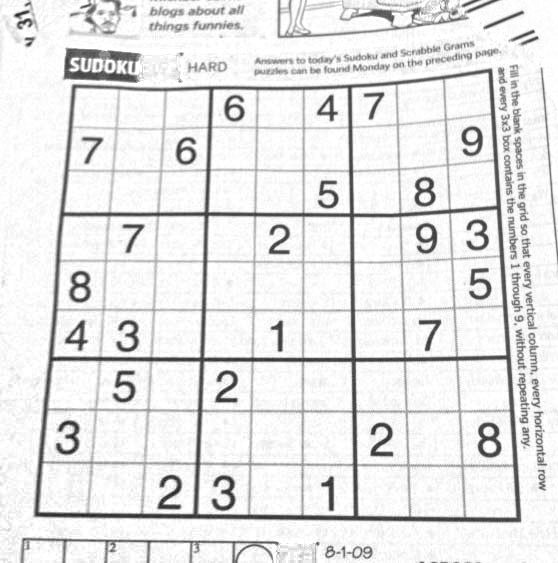
\includegraphics[height=.15\textheight]{./figure/sudoku.png}
			\caption{\texttt{sudoku.png}原图}
		\end{subfigure}
		\begin{subfigure}{.45\textwidth}
			\centering
			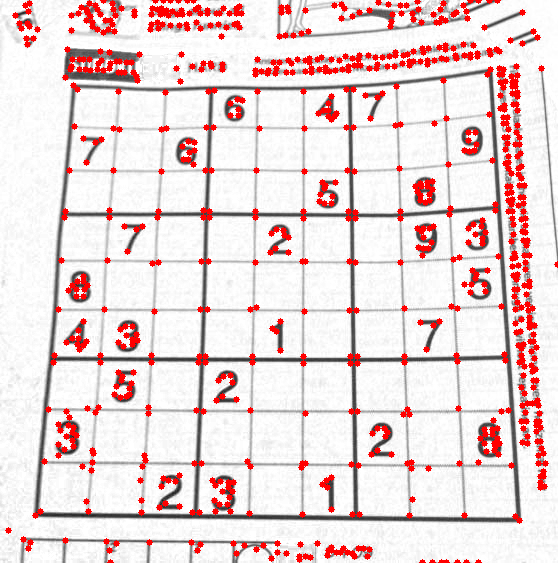
\includegraphics[height=.15\textheight]{./figure/sudoku_keypoints.png}
			\caption{检测角点}
		\end{subfigure}
		\caption{\texttt{sudoku.png}角点检测}
	\end{figure}
	
	此外,为了进一步评估 Harris 角点检测在复杂场景中的适用性,我们将该算法应用于包含丰富纹理和结构信息的 \verb|uttower.jpg| 图像。在该实验中,Harris 角点检测依然展现出良好的角点提取能力,能够在图像中的建筑边缘、窗口框架以及其他具有明显角点特征的区域成功识别出大量有效角点。实验结果表明,该方法在复杂背景下仍然具有较强的角点检测能力,能够较好地适应不同图像内容的变化。
	
	\begin{figure}[htbp]
		\centering
		\begin{subfigure}{.45\textwidth}
			\centering
			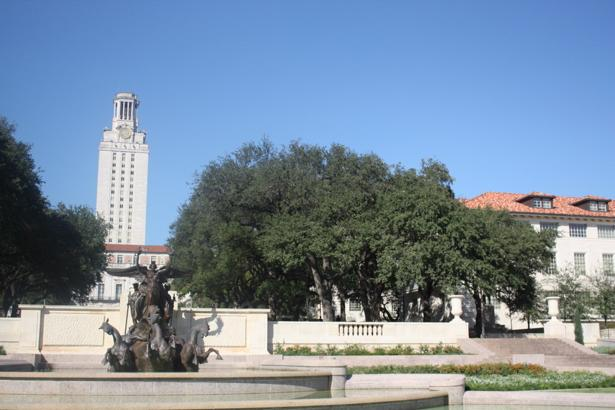
\includegraphics[height=.15\textheight]{./figure/uttower1.jpg}
			\caption{\texttt{uttower1.jpg}原图}
		\end{subfigure}
		\begin{subfigure}{.45\textwidth}
			\centering
			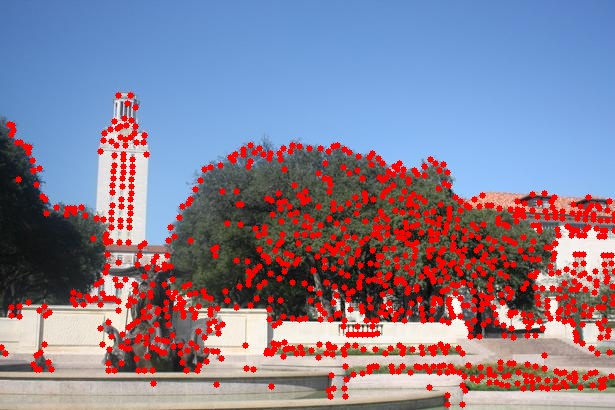
\includegraphics[height=.15\textheight]{./figure/uttower1_keypoints.jpg}
			\caption{检测角点}
		\end{subfigure}
		
		\begin{subfigure}{.45\textwidth}
			\centering
			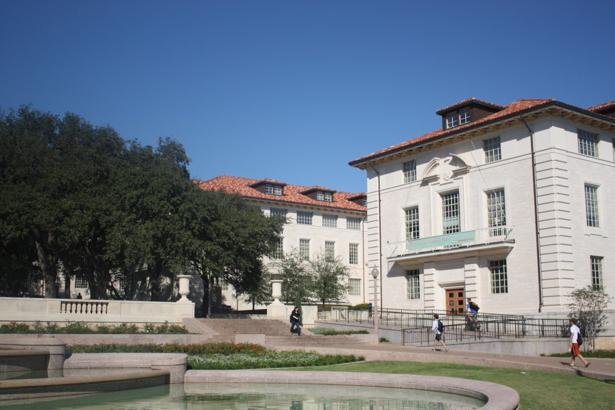
\includegraphics[height=.15\textheight]{./figure/uttower2.jpg}
			\caption{\texttt{uttower2.jpg}原图}
		\end{subfigure}
		\begin{subfigure}{.45\textwidth}
			\centering
			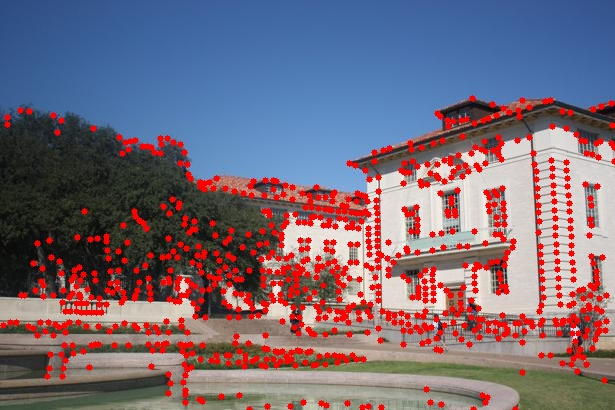
\includegraphics[height=.15\textheight]{./figure/uttower2_keypoints.jpg}
			\caption{检测角点}
		\end{subfigure}
		\caption{\texttt{uttower.jpg}角点检测}
	\end{figure}
	
	综合实验结果分析,Harris 角点检测方法在规则网格结构和自然场景图像中均能较好地完成角点检测任务,特别是在具有显著灰度梯度变化的区域表现优异。然而,该方法对于角点响应的稳定性仍然受到图像噪声和尺度变化的影响,这也是后续研究中需要进一步优化的方向。
	
	\subsection{图像拼接对比实验}
	
	在本部分实验中,我们首先对比了自主编写的 HOG 特征匹配函数与 OpenCV 自带 HOG 特征匹配函数在 uttower.jpg 图像上的效果。从实验结果来看,自编写的特征匹配函数仅能成功匹配部分主要特征点,而忽略了许多潜在的匹配特征点。这种匹配能力的局限性主要源于两个方面的因素:首先,自主编写的 HOG 特征计算可能未能充分提取梯度方向直方图信息,导致特征描述子维度不够完整,从而降低了匹配的准确性;其次,在匹配策略上,自编写的版本可能缺乏高效的最近邻搜索和筛选机制,导致匹配结果较为稀疏。而 OpenCV 版本的 HOG 特征计算充分考虑了局部梯度方向变化,并结合优化后的特征匹配策略,从而能够提取更多关键特征,并在匹配过程中保留更具区分度的特征点对,提高了整体匹配的完整性和鲁棒性。
	
	\begin{figure}[htbp]
		\centering
		\begin{subfigure}{.8\textwidth}
			\centering
			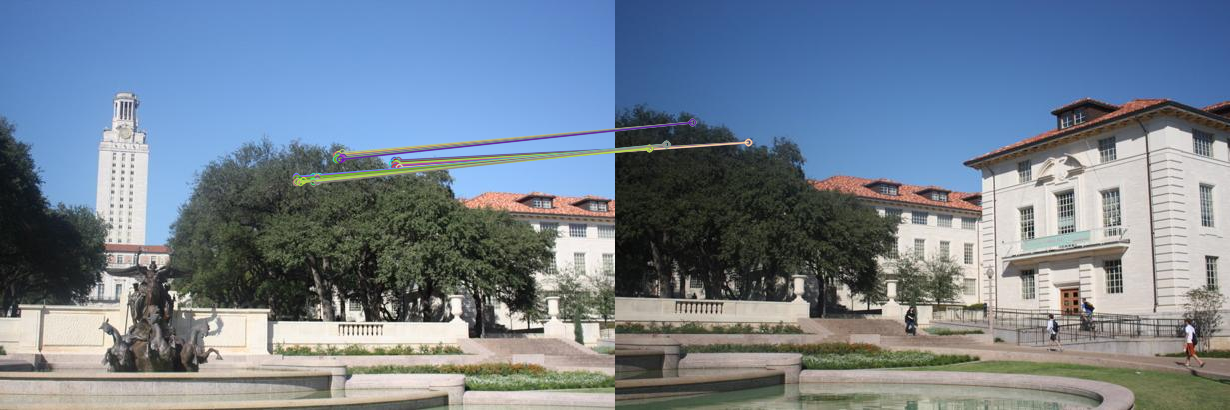
\includegraphics[height=.15\textheight]{./figure/uttower_handon_match_hog.png}
			\caption{自写HOG方法特征子匹配}
		\end{subfigure}
		\begin{subfigure}{.8\textwidth}
			\centering
			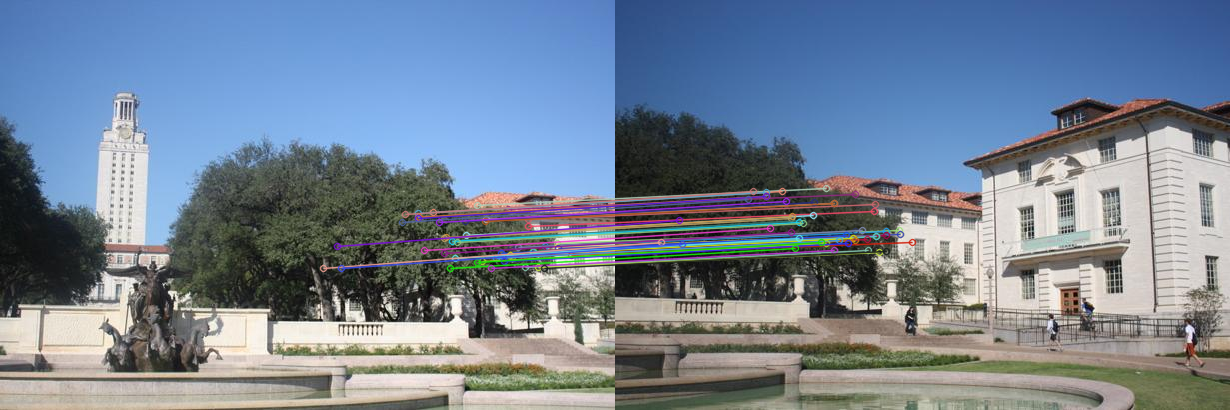
\includegraphics[height=.15\textheight]{./figure/uttower_opencv_match_hog.png}
			\caption{Opencv\ HOG方法特征子匹配}
		\end{subfigure}
		
		\begin{subfigure}{.45\textwidth}
			\centering
			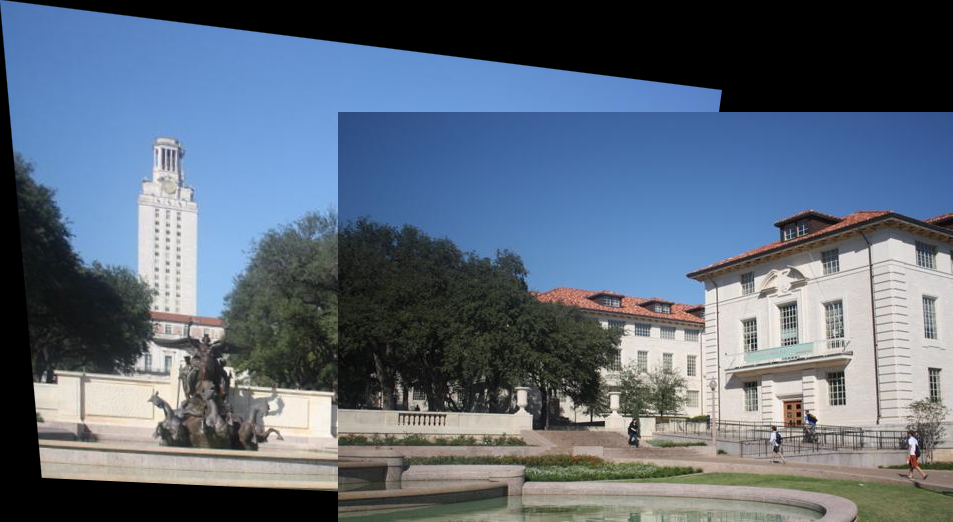
\includegraphics[height=.13\textheight]{./figure/uttower_handon_stitching_hog.png}
			\caption{自写HOG方法图像拼接}
		\end{subfigure}
		\begin{subfigure}{.45\textwidth}
			\centering
			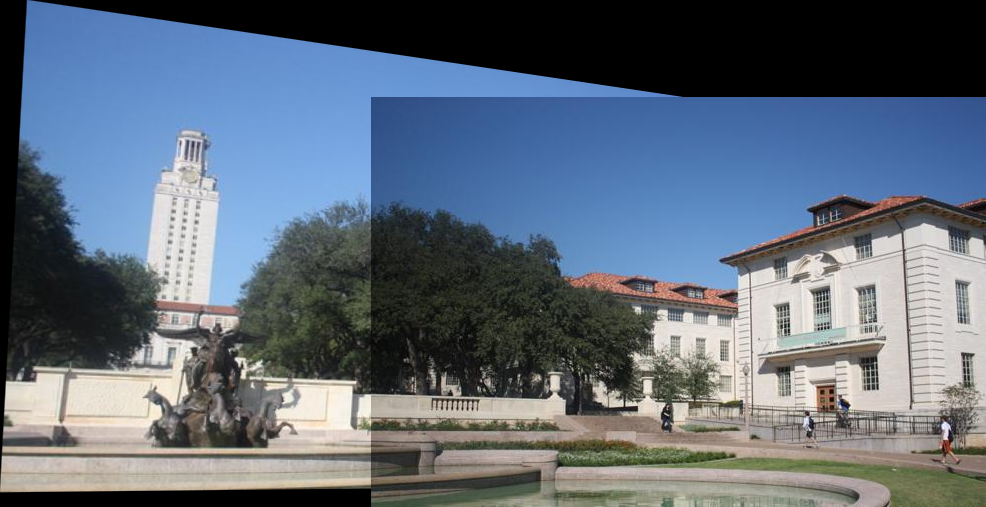
\includegraphics[height=.13\textheight]{./figure/uttower_opencv_stitching_hog.png}
			\caption{Opencv\ HOG方法图像拼接}
		\end{subfigure}
		\caption{HOG特征子匹配实验}
	\end{figure}

	随后,我们对比了 SIFT 特征检测与匹配的三种实现版本,即自主编写的 SIFT 版本、自主优化的 SIFT 版本以及 OpenCV 自带的 SIFT 版本,并在 \verb|uttower.jpg| 图像上进行了实验。实验结果表明,未经优化的自主编写 SIFT 方法在检测和匹配方面表现较差,匹配点较少且精度较低。这主要是由于自编写版本在关键点尺度空间构建过程中可能未能充分考虑尺度归一化,导致关键点检测不稳定,同时梯度直方图计算和关键点描述子生成过程中插值方式的缺失,影响了最终的匹配效果。而在优化后,自主优化版本的 SIFT 通过引入高斯加权梯度计算、双线性插值等改进策略,有效提升了关键点描述子的稳定性和匹配精度,从而使得最终的匹配结果与 OpenCV 版本的 SIFT 结果基本一致,仅在部分特征点的匹配上存在细微差异,但整体拼接效果已基本无明显差别。
	
	\begin{figure}[htbp]
		\centering
		\begin{subfigure}{.8\textwidth}
			\centering
			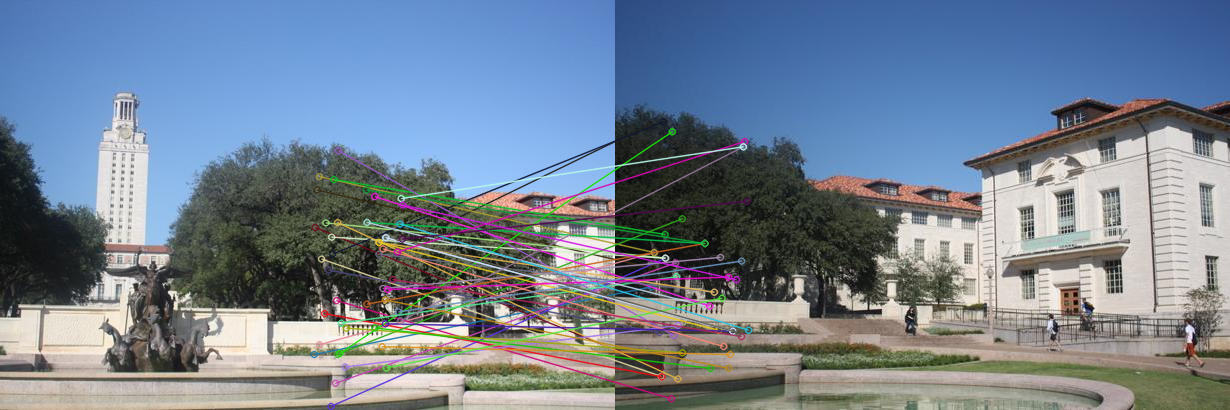
\includegraphics[height=.13\textheight]{./figure/uttower_handon_match_sift.png}
			\caption{自写SIFT方法特征子匹配}
		\end{subfigure}
		\begin{subfigure}{.8\textwidth}
			\centering
			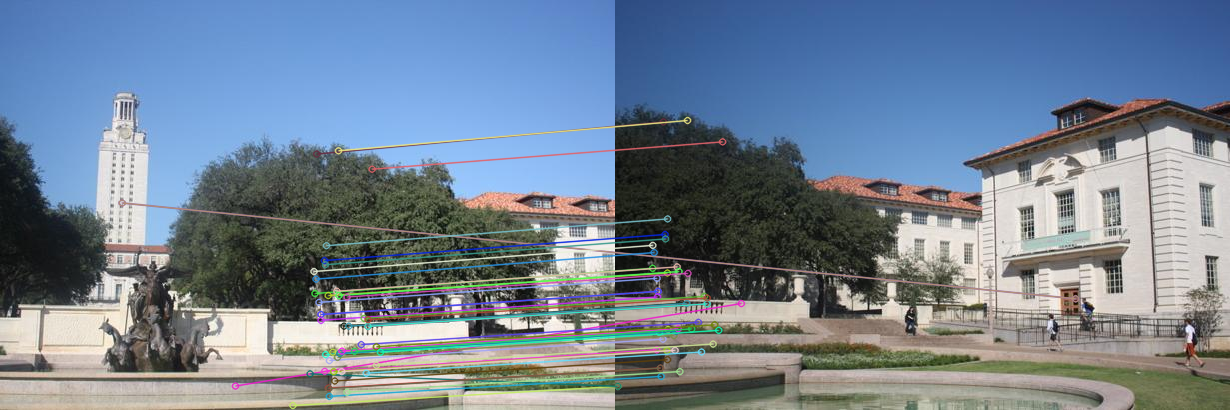
\includegraphics[height=.13\textheight]{./figure/uttower_handon_match_sift_opt.png}
			\caption{优化SIFT方法特征子匹配}
		\end{subfigure}
		\begin{subfigure}{.8\textwidth}
			\centering
			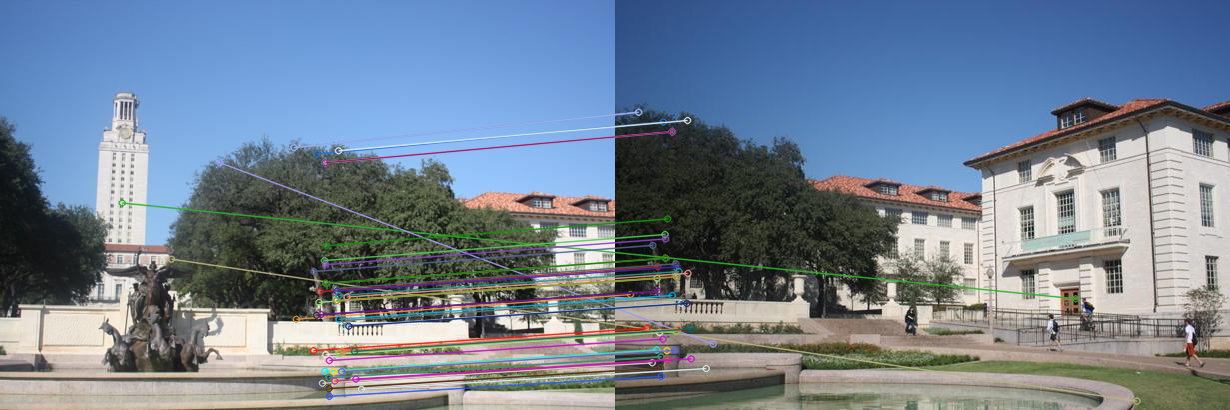
\includegraphics[height=.13\textheight]{./figure/uttower_opencv_match_sift.png}
			\caption{Opencv\ SIFT方法特征子匹配}
		\end{subfigure}
		
		\begin{subfigure}{.27\textwidth}
			\centering
			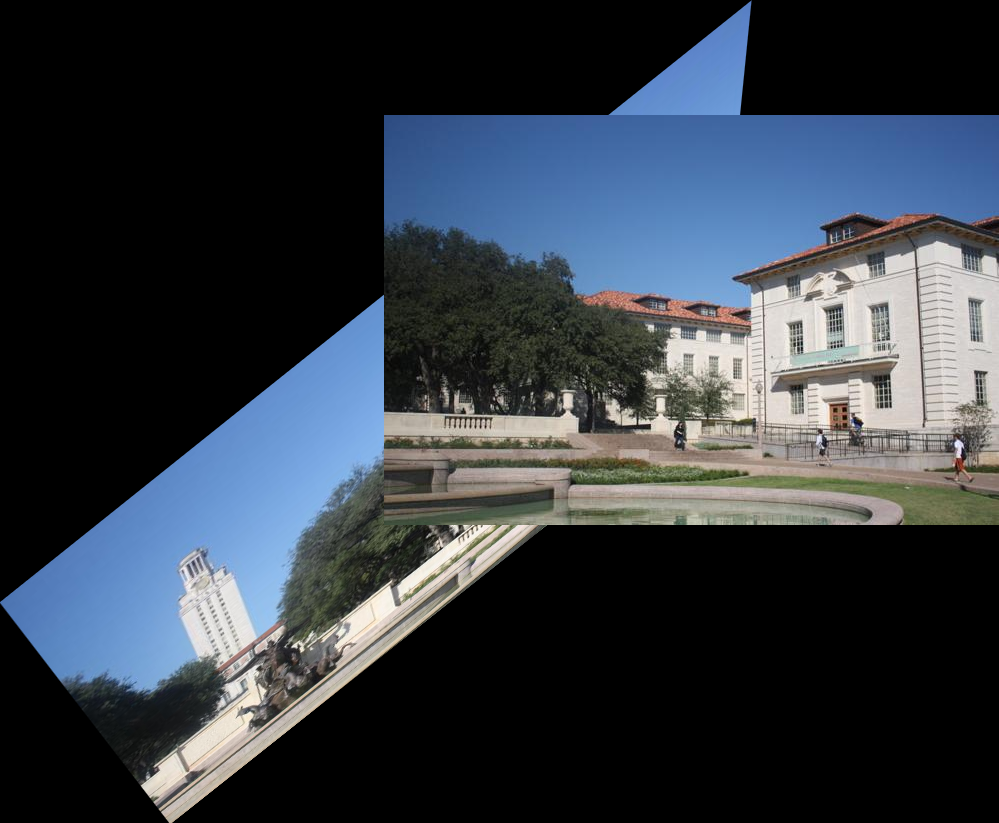
\includegraphics[height=.1\textheight]{./figure/uttower_handon_stitching_sift.png}
			\caption{自写SIFT方法图像拼接}
		\end{subfigure}
		\begin{subfigure}{.35\textwidth}
			\centering
			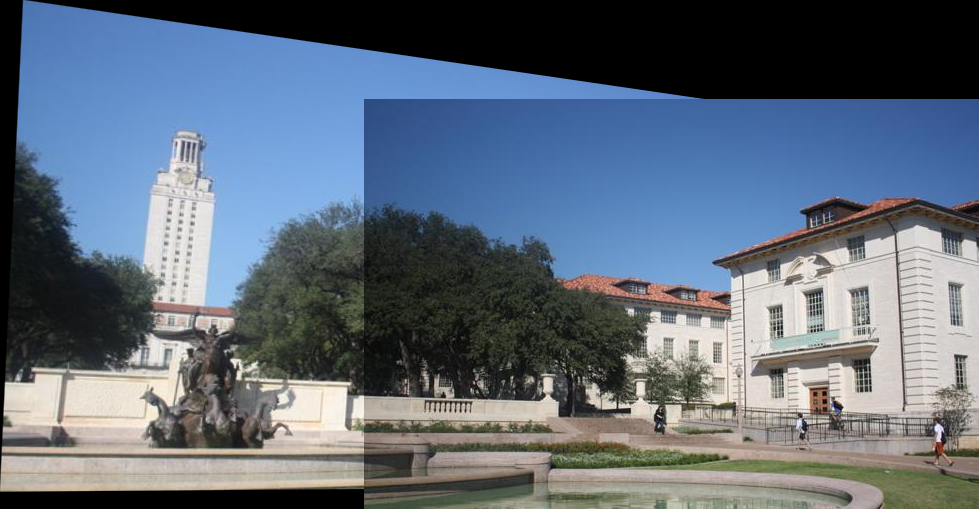
\includegraphics[height=.1\textheight]{./figure/uttower_handon_stitching_sift_opt.png}
			\caption{优化SIFT方法图像拼接}
		\end{subfigure}
		\begin{subfigure}{.35\textwidth}
			\centering
			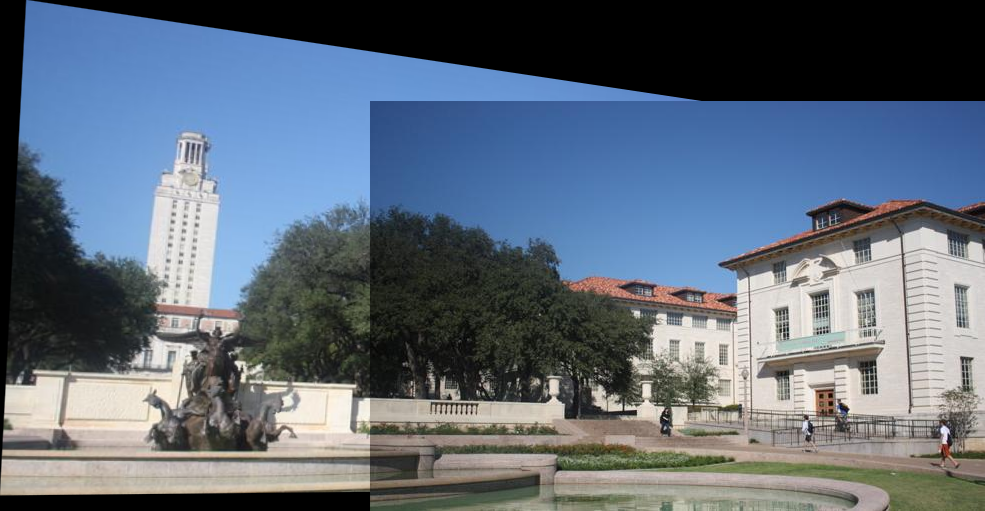
\includegraphics[height=.1\textheight]{./figure/uttower_opencv_stitching_sift.png}
			\caption{Opencv\ SIFT方法图像拼接}
		\end{subfigure}
		\caption{SIFT特征子匹配实验}
	\end{figure}

	接着,我们对比了 HOG 和 SIFT 方法在图像拼接任务中的表现。实验结果显示,两种方法在拼接 \verb|uttower.jpg| 时,最终的拼接效果大体一致,但在细节匹配精度上存在一定差异。具体而言,HOG 方法由于主要依赖局部梯度方向变化来进行特征提取,在处理结构化明显的区域(如建筑轮廓、窗口边缘)时具有较好的表现,但在缺乏明显梯度变化的平坦区域(如白墙面)上,HOG 无法提供足够的角点信息,导致特征点提取不足,从而影响匹配质量。而 SIFT 由于采用尺度空间检测方式,并结合 DoG(差分高斯)进行关键点提取,能够在较大范围内捕捉到稳定的特征点,即使在纹理较少的区域,也能够提取一定程度上的特征点。因此,整体而言,HOG 方法在结构化明显的区域表现较好,但在白墙等低纹理区域的角点检测能力不及 SIFT,导致拼接结果在这些区域的匹配精度略逊于 SIFT 方法。

	最后,我们将 SIFT 特征检测与 RANSAC 进行结合,以完成更大尺度的全景拼接实验。本次实验选用了 \verb|yosemite.jpg| 图像,并利用 SIFT 提取关键点,随后通过 RANSAC 估算单应性矩阵,最终完成图像的拼接。从实验结果来看,最终的拼接结果十分理想,能够准确对齐多个图像的对应区域,实现了无缝的拼接效果,符合实验预期。这一结果进一步验证了 SIFT 特征匹配的鲁棒性以及 RANSAC 在去除误匹配点对中的有效性,为后续更复杂的全景拼接任务提供了可靠的技术支持。
	
	\begin{figure}[htbp]
		\centering
		\begin{subfigure}{.45\textwidth}
			\centering
			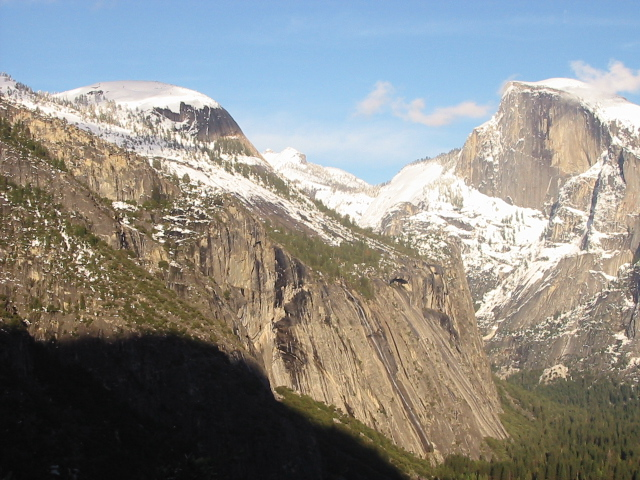
\includegraphics[height=.13\textheight]{./figure/yosemite1.jpg}
			\caption{\texttt{yosemite1.jpg}原图}
		\end{subfigure}
		\begin{subfigure}{.45\textwidth}
			\centering
			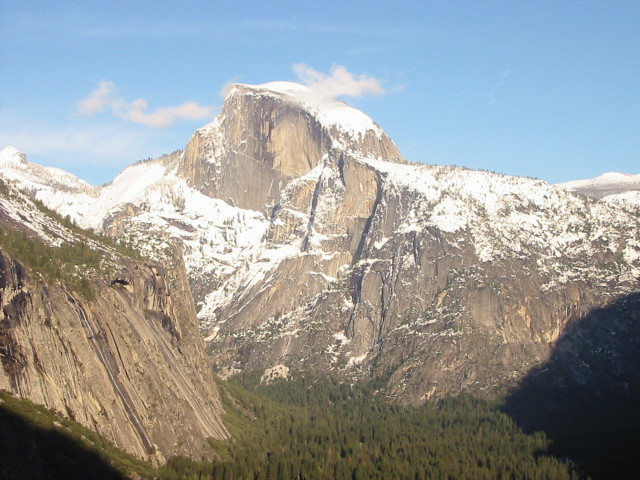
\includegraphics[height=.13\textheight]{./figure/yosemite2.jpg}
			\caption{\texttt{yosemite2.jpg}原图}
		\end{subfigure}
		
		\begin{subfigure}{.45\textwidth}
			\centering
			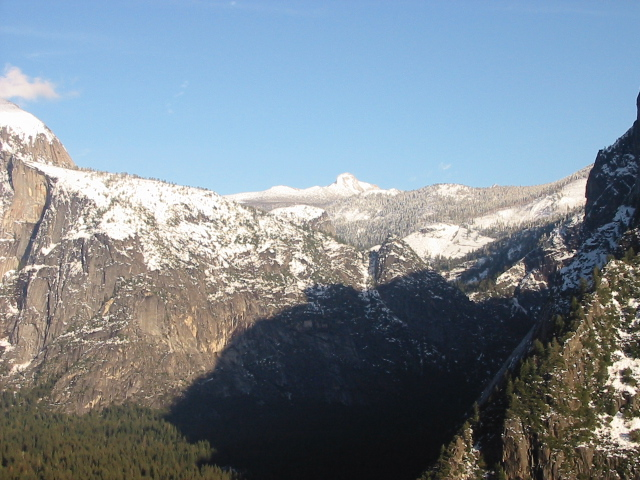
\includegraphics[height=.13\textheight]{./figure/yosemite3.jpg}
			\caption{\texttt{yosemite3.jpg}原图}
		\end{subfigure}
		\begin{subfigure}{.45\textwidth}
			\centering
			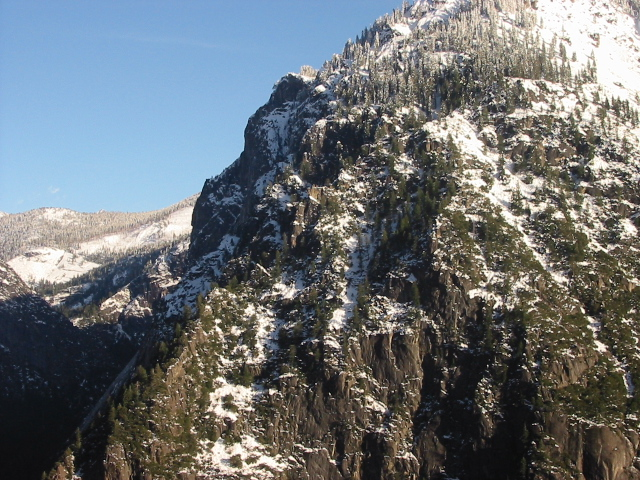
\includegraphics[height=.13\textheight]{./figure/yosemite4.jpg}
			\caption{\texttt{yosemite4.jpg}原图}
		\end{subfigure}
		
		\begin{subfigure}{.8\textwidth}
			\centering
			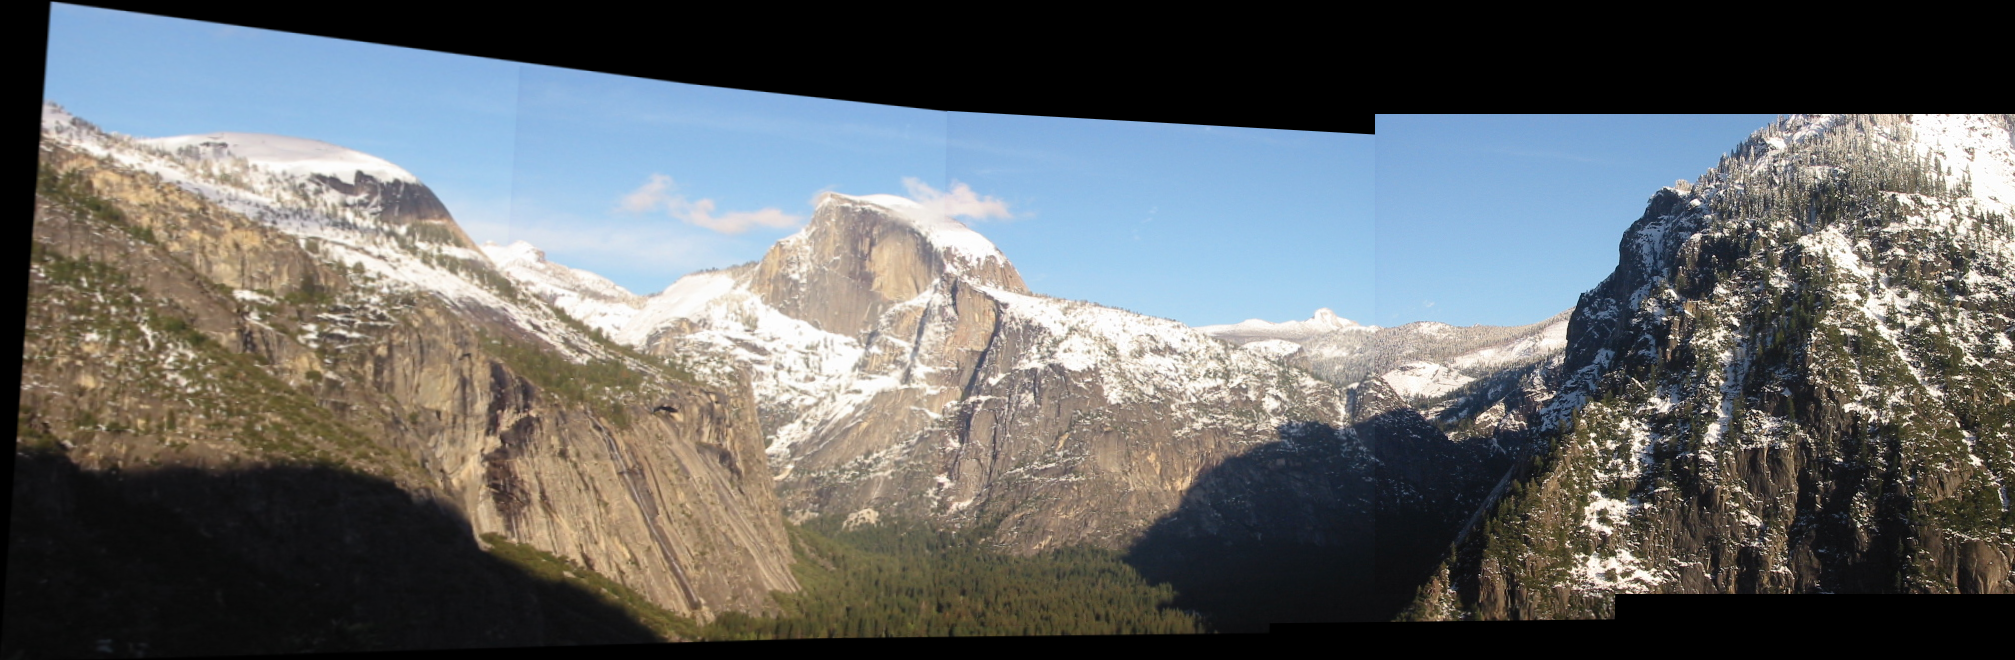
\includegraphics[height=.13\textheight]{./figure/yosemite_opencv_stitching.png}
			\caption{\texttt{yosemite.jpg}拼接图像}
		\end{subfigure}
		\caption{SIFT算法及RANSAC算法的图像拼接}
	\end{figure}
	
	\subsection{图像配准应用实验}
	
	在图像配准任务中,如果基于关键点并依据关键点匹配结果进行配准,我们通常称其为端对端配准方案 \cite{reg}。为了深入检验 SIFT 特征匹配与 RANSAC 估计方法在医学图像配准中的实际应用效果,本实验选取了 RIRE(Retrospective Image Registration Evaluation)数据集,并选用了其中同一病人的头部 MRI T1 加权图像与 MRI T2 加权图像作为实验对象。通过 SIFT 提取两幅图像的关键点,并利用 RANSAC 进行单应性矩阵估计,实现配准变换,最终对配准结果进行可视化分析与评估。实验结果表明,该方法在病人头部的下半部分(如颅底与颅骨边缘)能够取得较好的配准效果,关键解剖结构在配准后能够基本对齐。然而,在大脑区域的配准结果仍然存在一定程度的误差,主要体现在关键点匹配数量较少以及部分匹配点的误差较大,导致变换矩阵无法准确描述两幅图像的几何关系,从而影响整体配准精度。  
	
	这一问题的根源在于 SIFT 算法在处理医学图像时的局限性。首先,医学图像(尤其是 MRI)通常存在较大的灰度不均衡问题,不同模态(如 T1 和 T2)之间的对比度差异较为显著,导致 SIFT 关键点检测器在不同模态图像上提取的特征点分布不一致,影响匹配的稳定性。其次,SIFT 依赖于梯度信息进行特征点提取,而医学图像中脑组织区域的梯度变化较为平滑,导致 SIFT 在该区域内提取的特征点较少,从而降低匹配点的数量。此外,RANSAC 算法在误匹配点较多的情况下,可能会受到误差影响,导致最终估计的单应性矩阵精度下降,影响整体配准质量。
	
	\begin{figure}[htbp]
		\centering
		\begin{subfigure}{.6\textwidth}
			\centering
			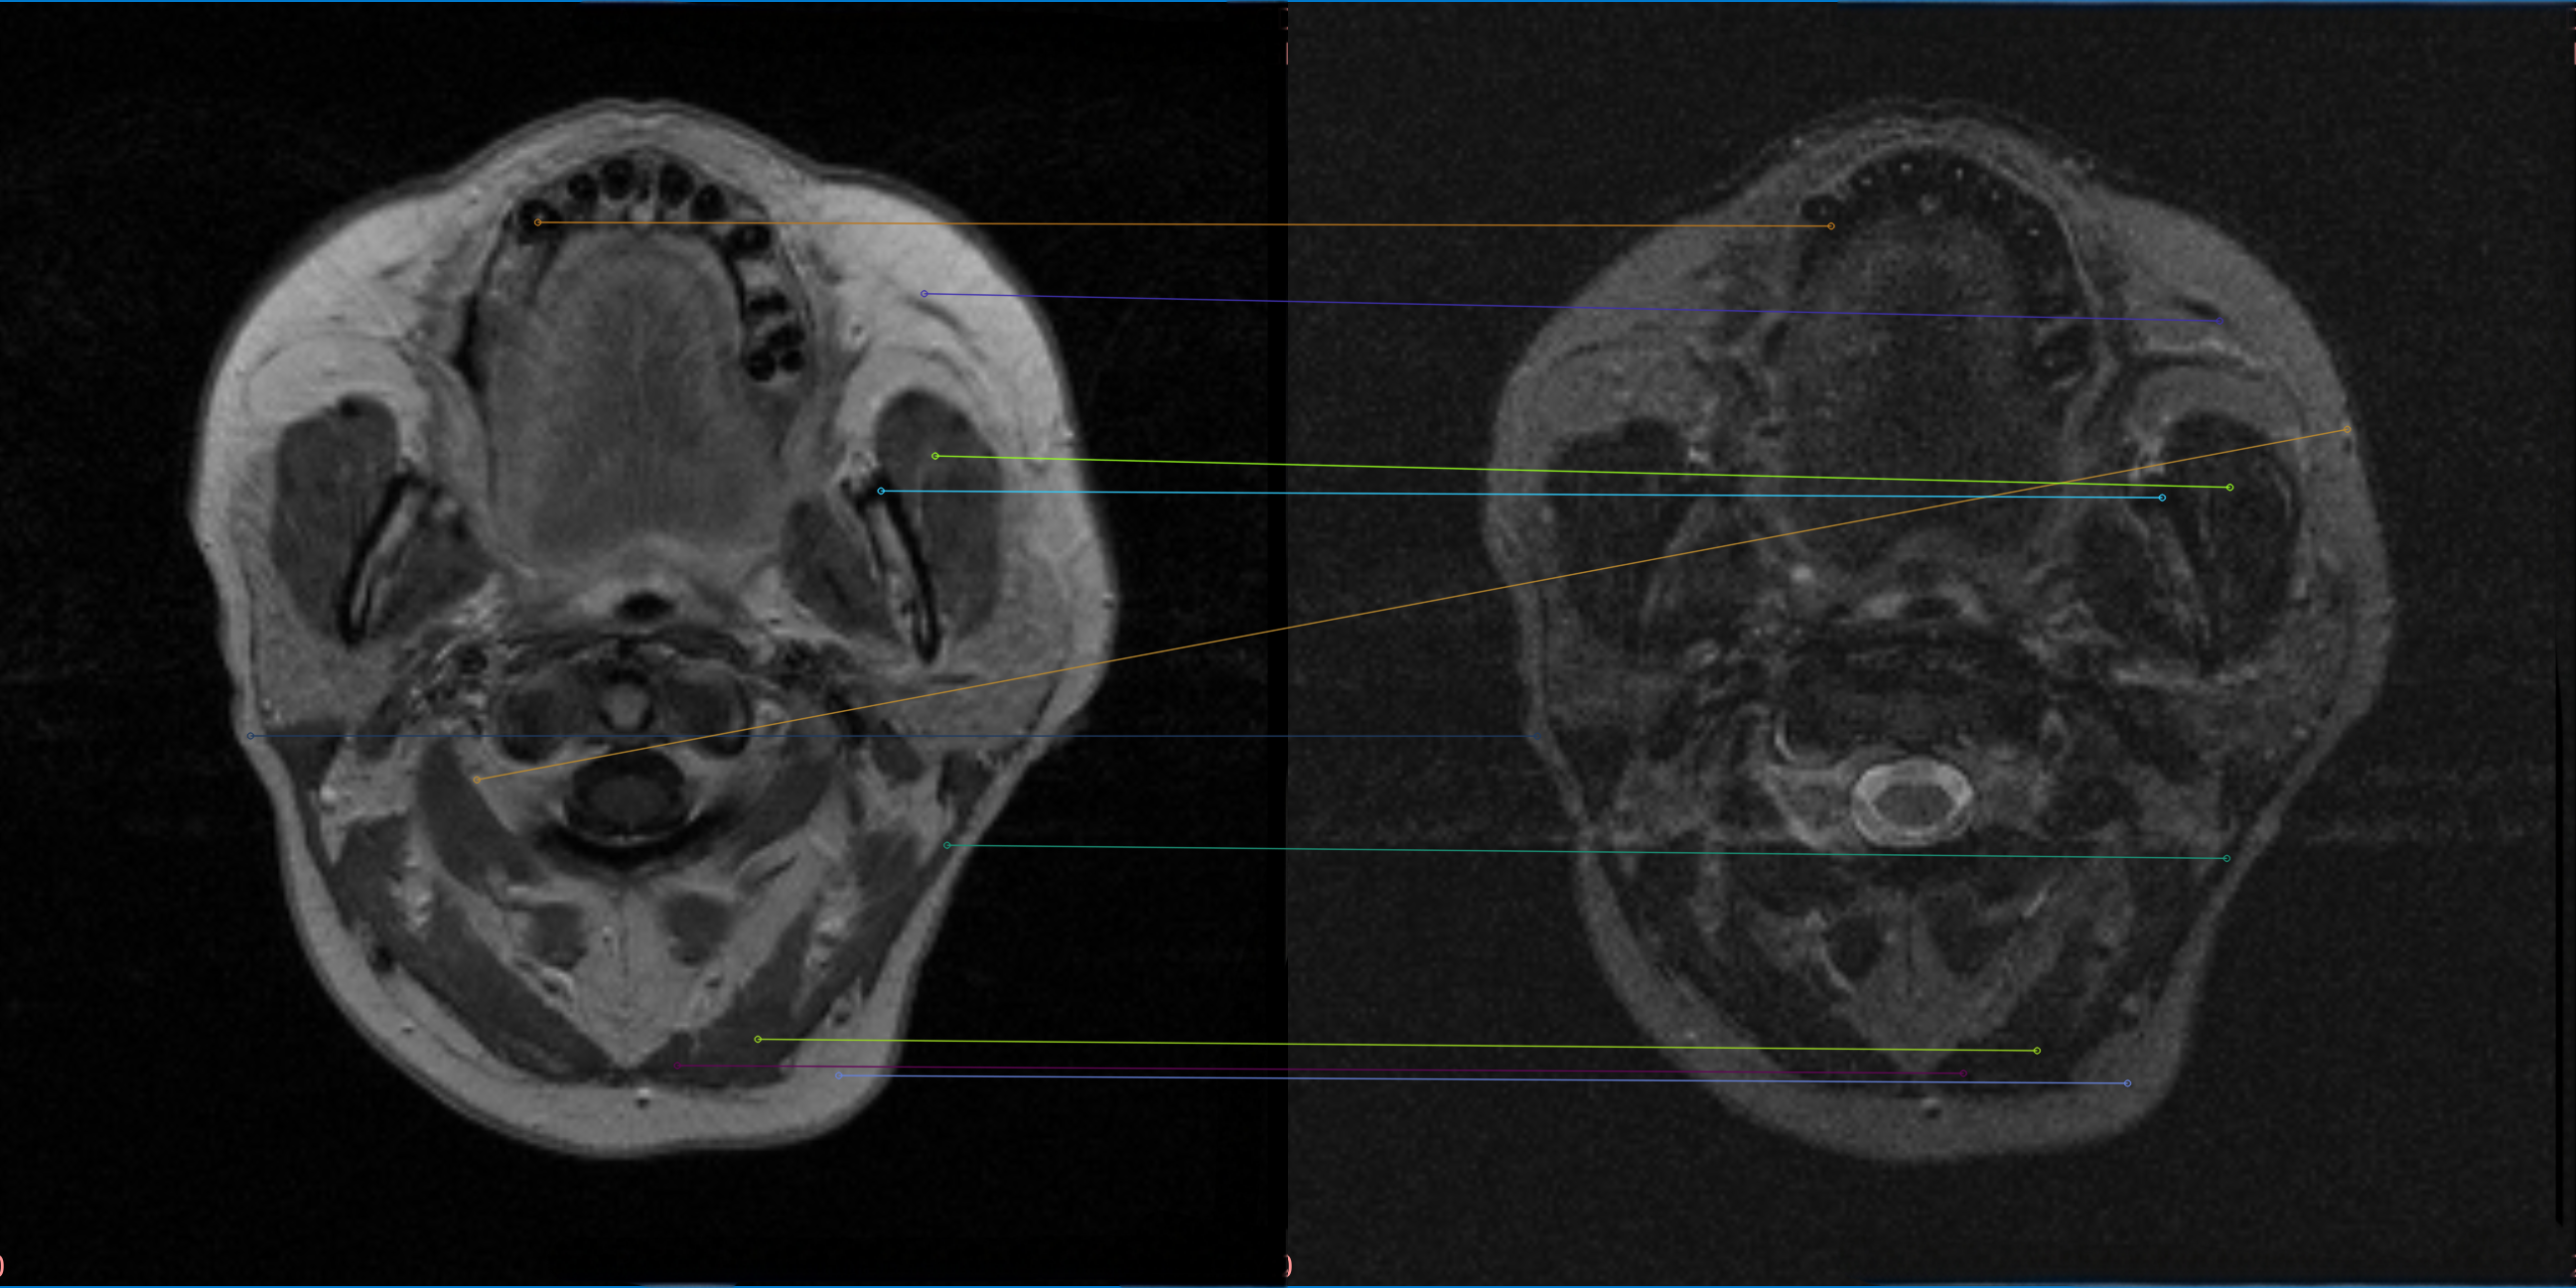
\includegraphics[height=.13\textheight]{./figure/match_opencv_1.png}
			\caption{病人断层图像关键点匹配1}
		\end{subfigure}
		\begin{subfigure}{.3\textwidth}
			\centering
			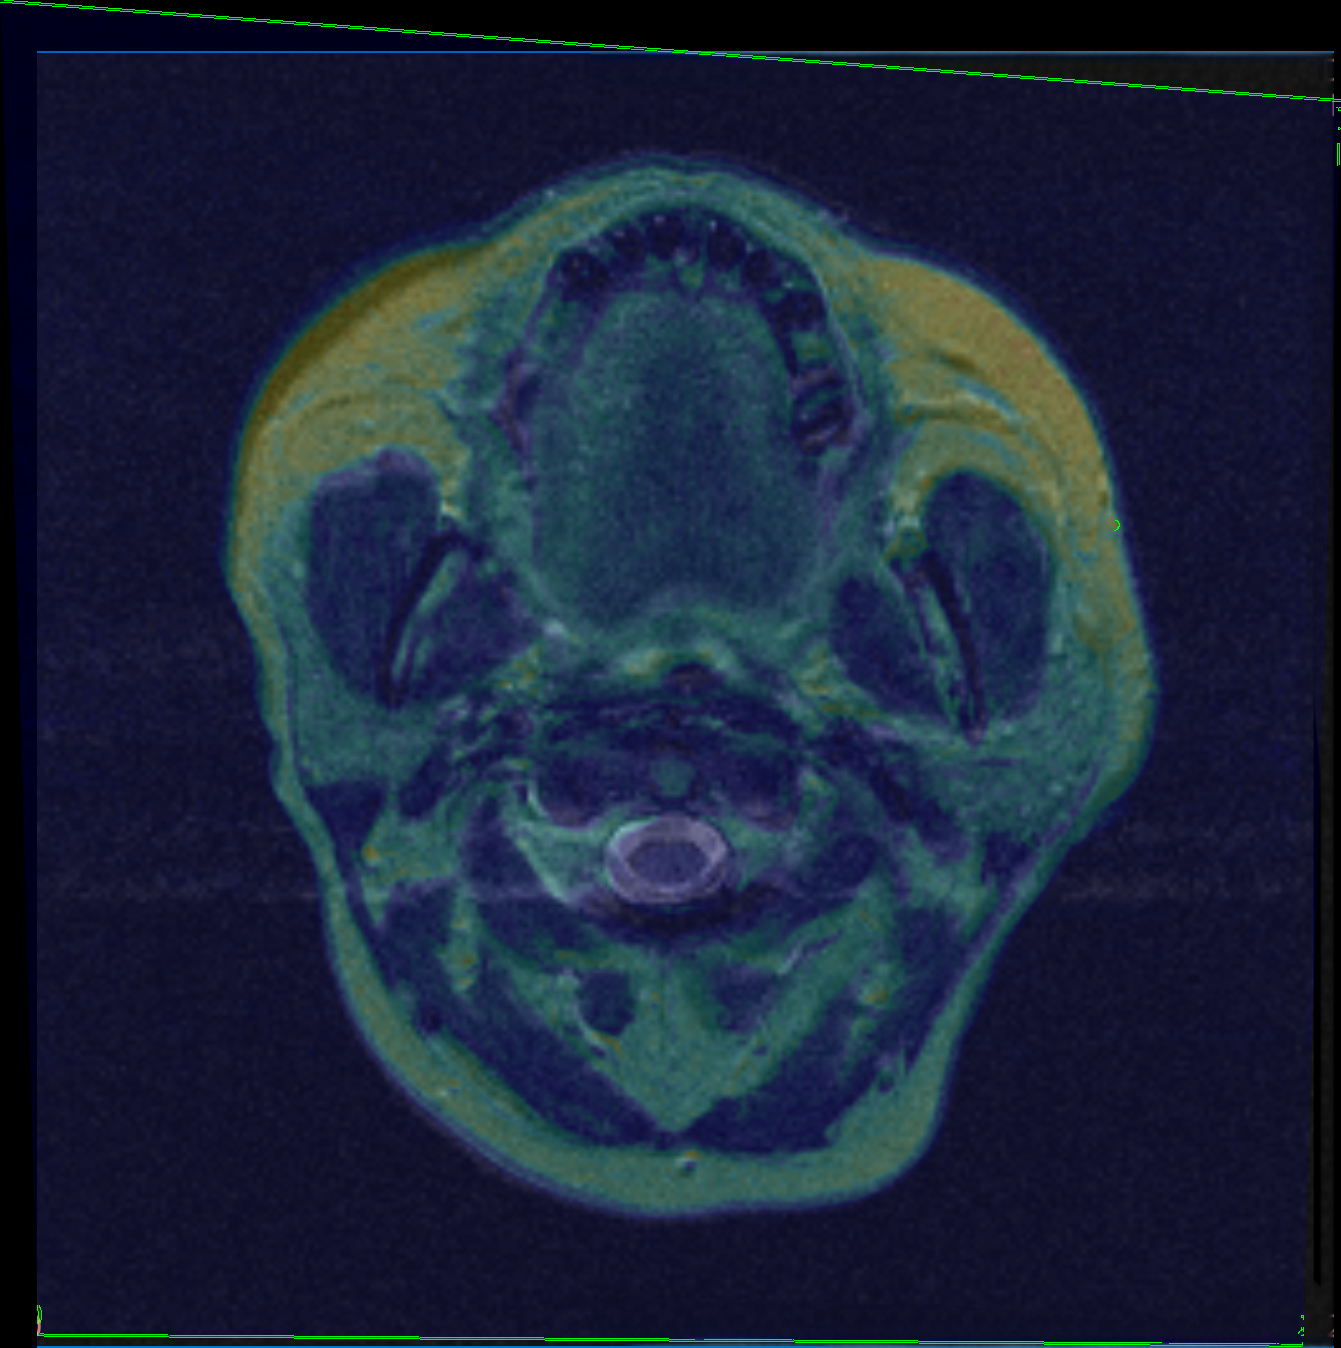
\includegraphics[height=.13\textheight]{./figure/compare_opencv_1.png}
			\caption{图像配准效果示意1}
		\end{subfigure}
		
		\begin{subfigure}{.6\textwidth}
			\centering
			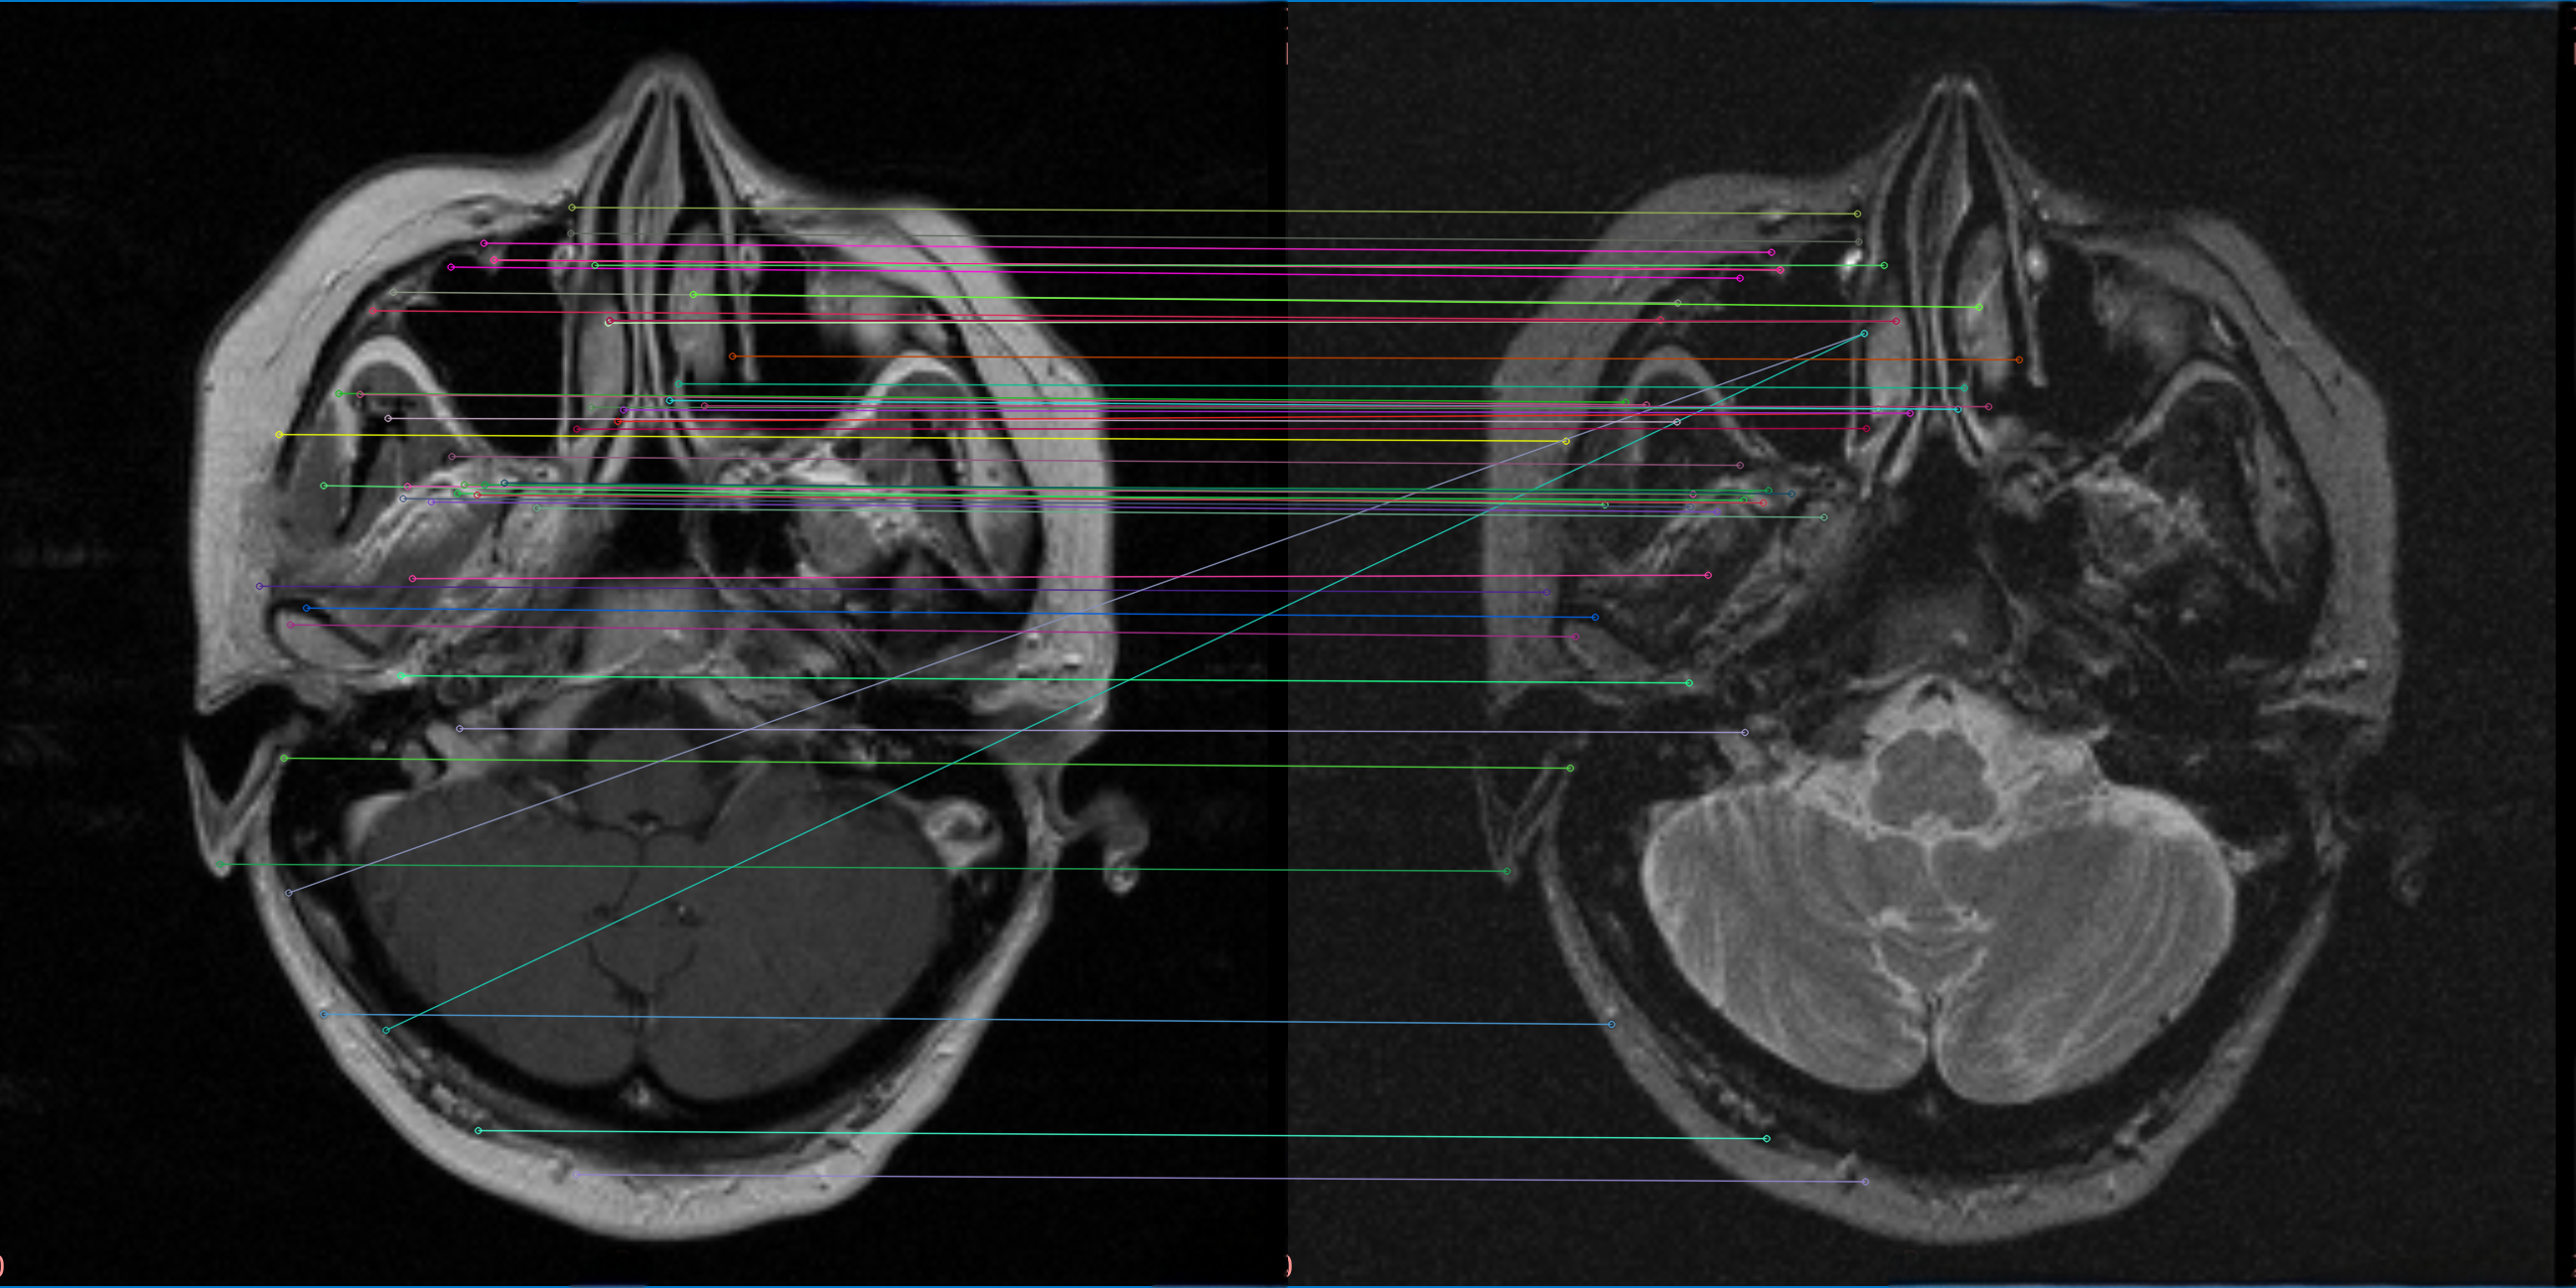
\includegraphics[height=.13\textheight]{./figure/match_opencv_2.png}
			\caption{病人断层图像关键点匹配2}
		\end{subfigure}
		\begin{subfigure}{.3\textwidth}
			\centering
			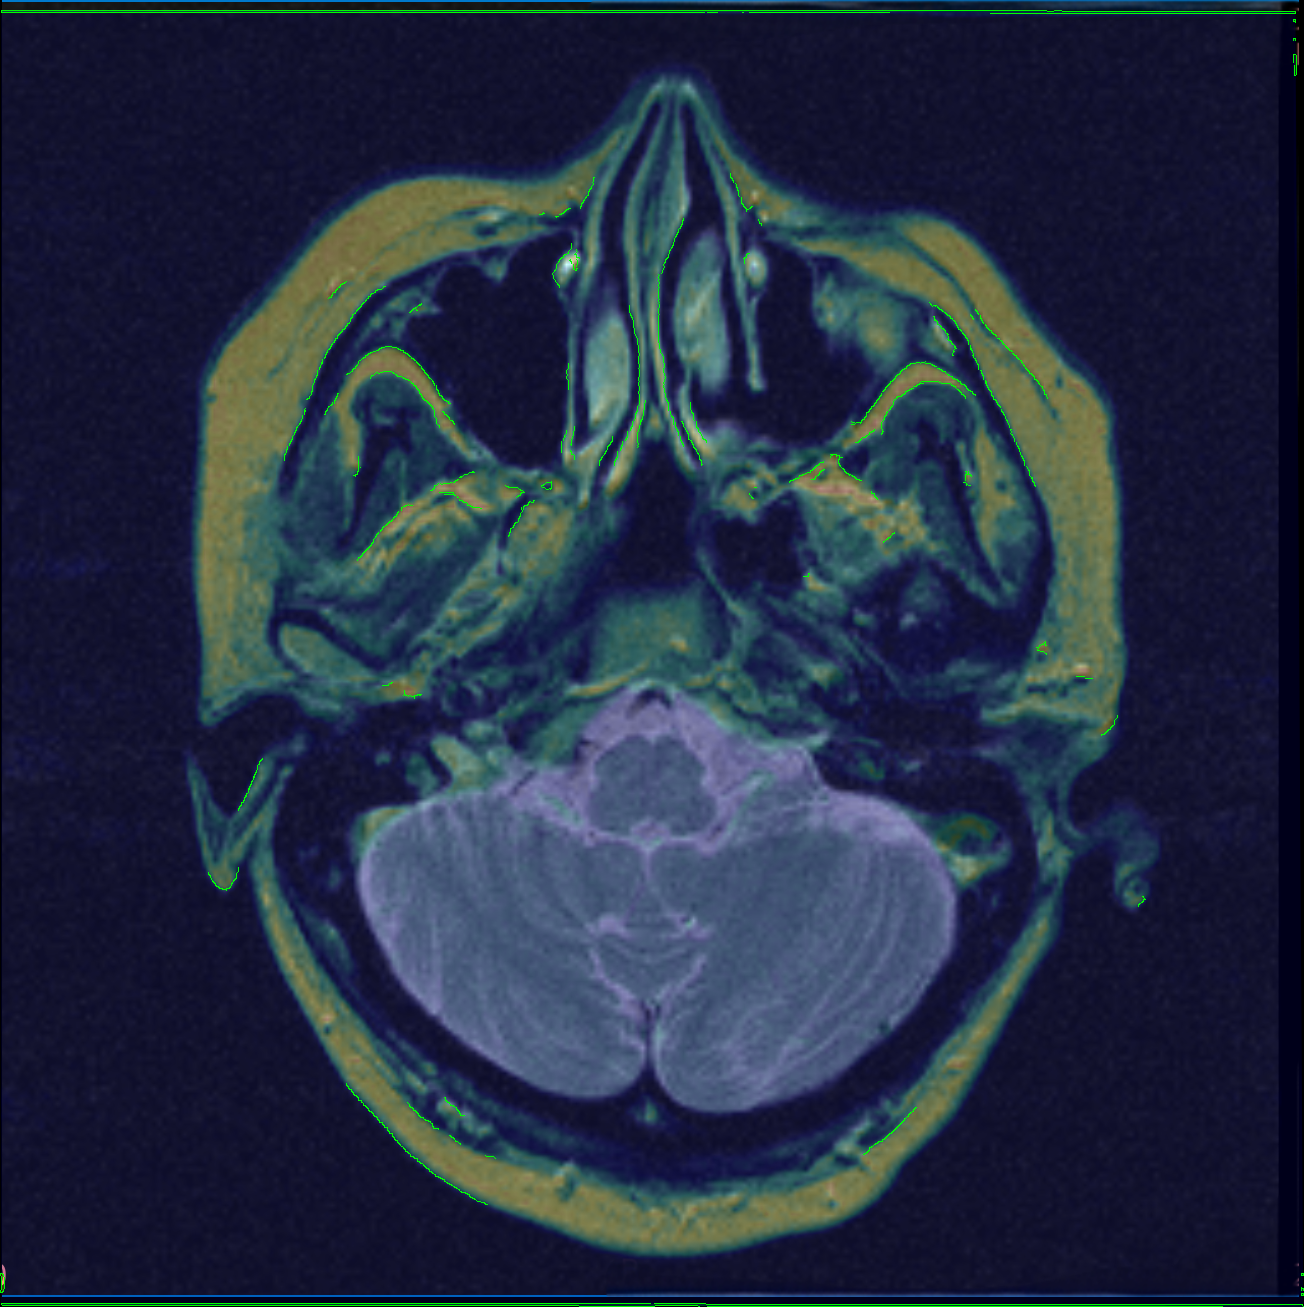
\includegraphics[height=.13\textheight]{./figure/compare_opencv_2.png}
			\caption{图像配准效果示意2}
		\end{subfigure}
		
		\begin{subfigure}{.6\textwidth}
			\centering
			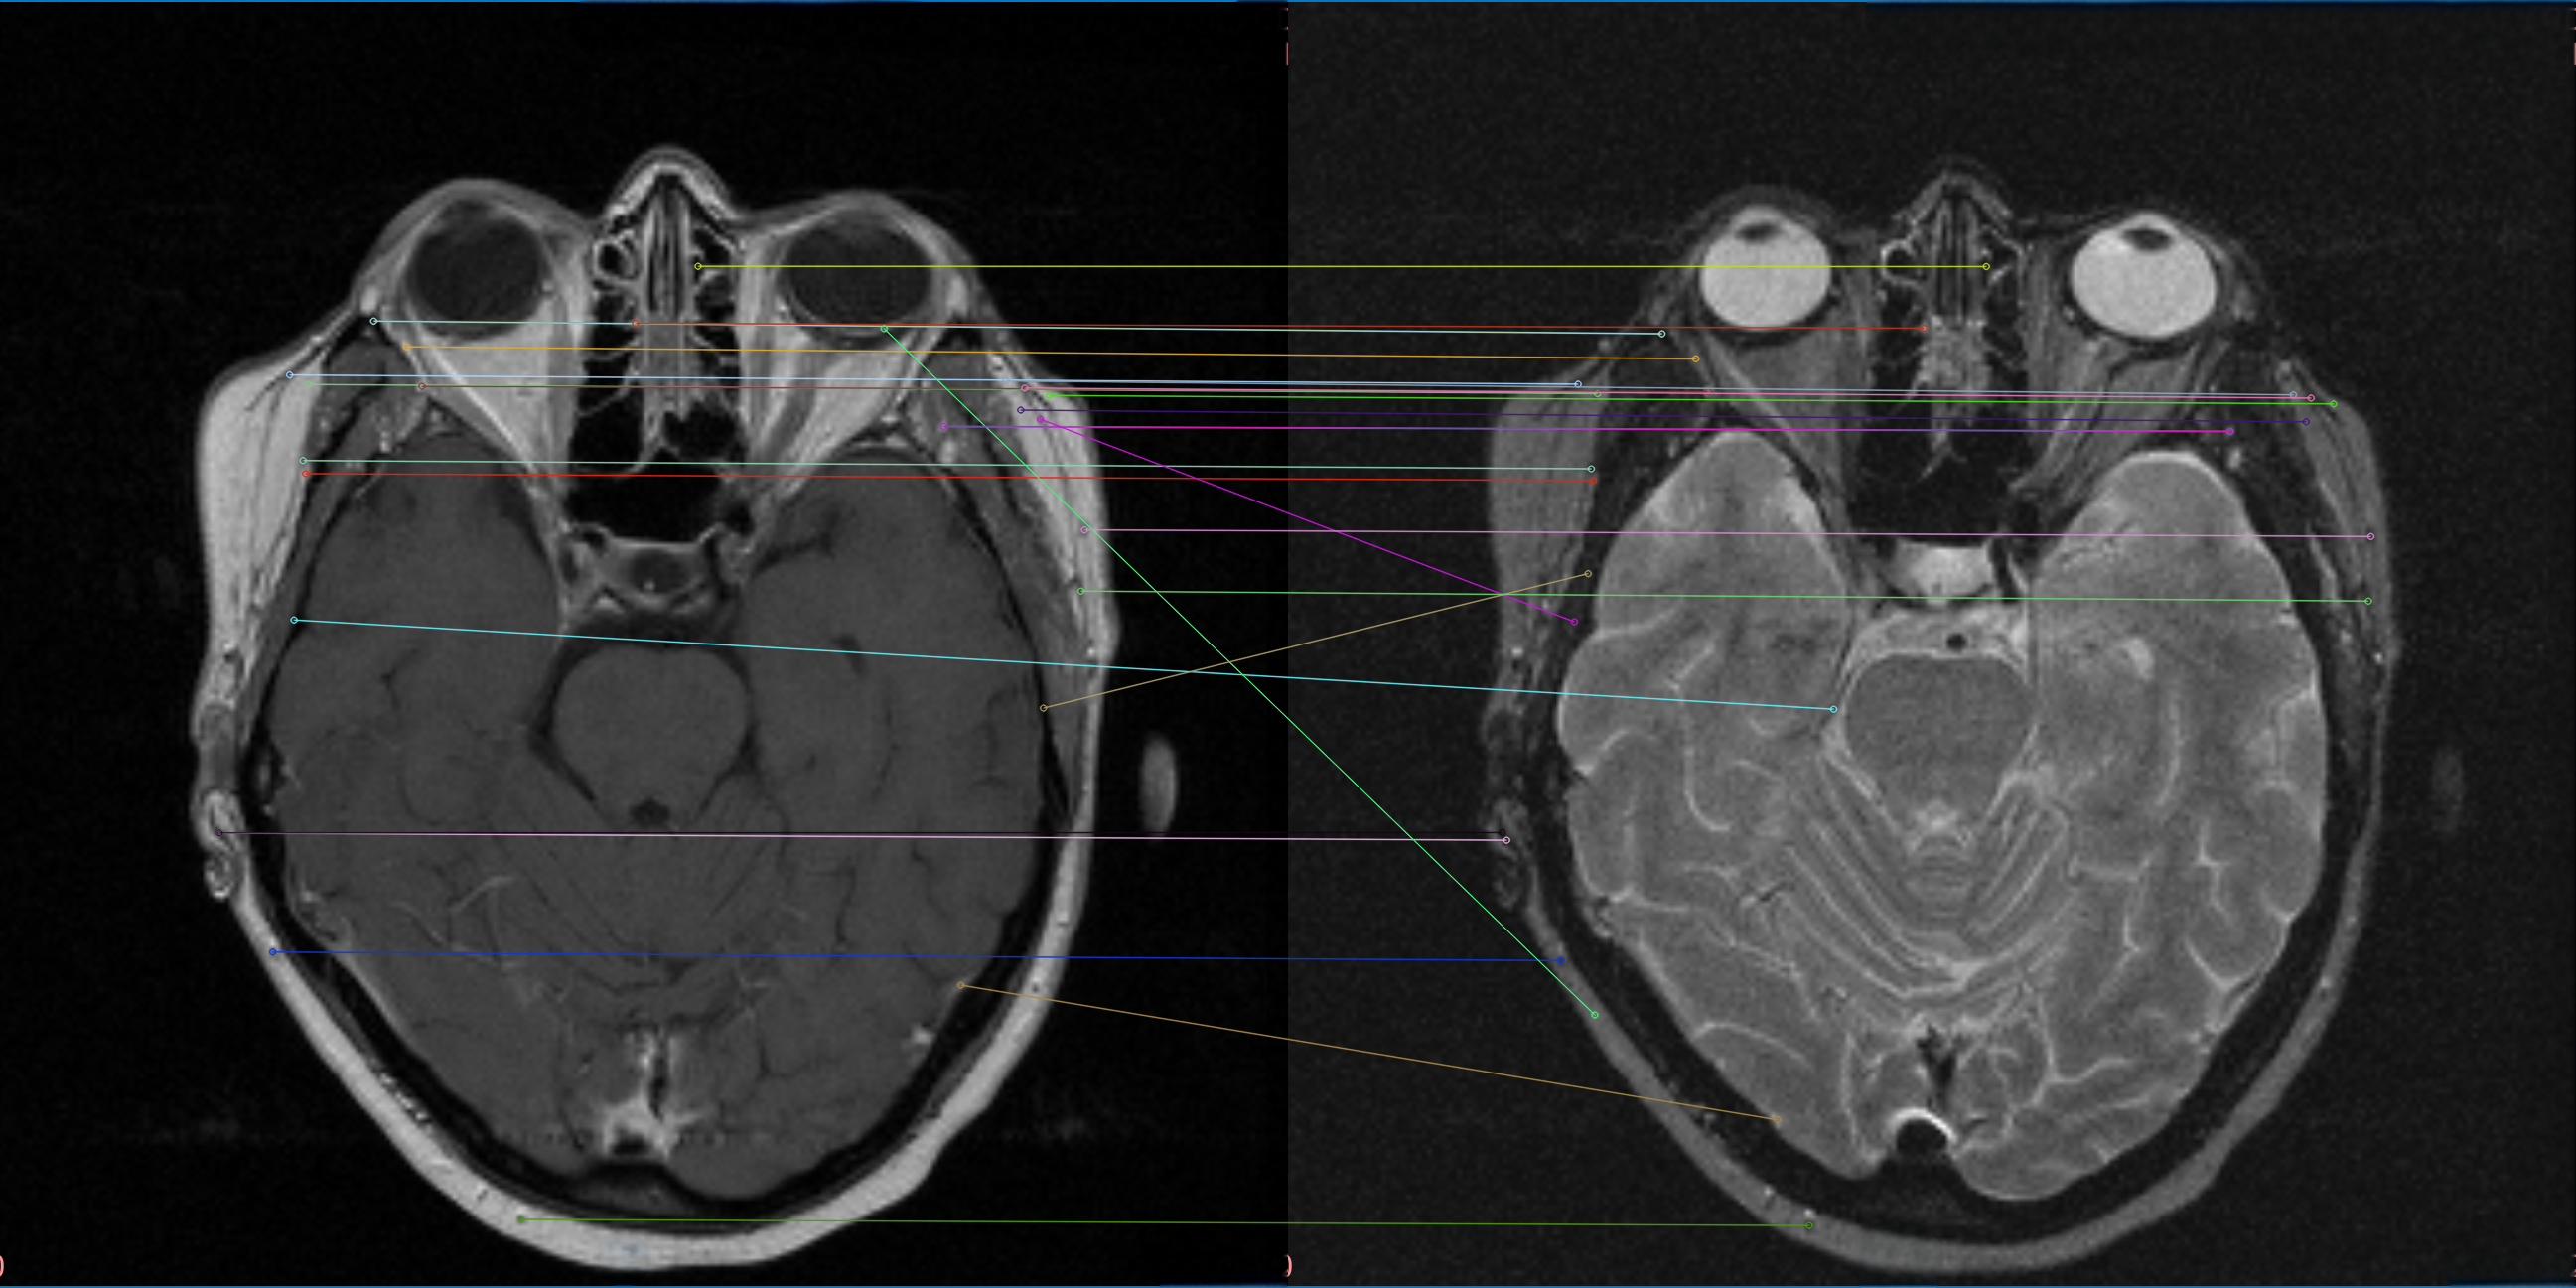
\includegraphics[height=.13\textheight]{./figure/match_opencv_3.png}
			\caption{病人断层图像关键点匹配3}
		\end{subfigure}
		\begin{subfigure}{.3\textwidth}
			\centering
			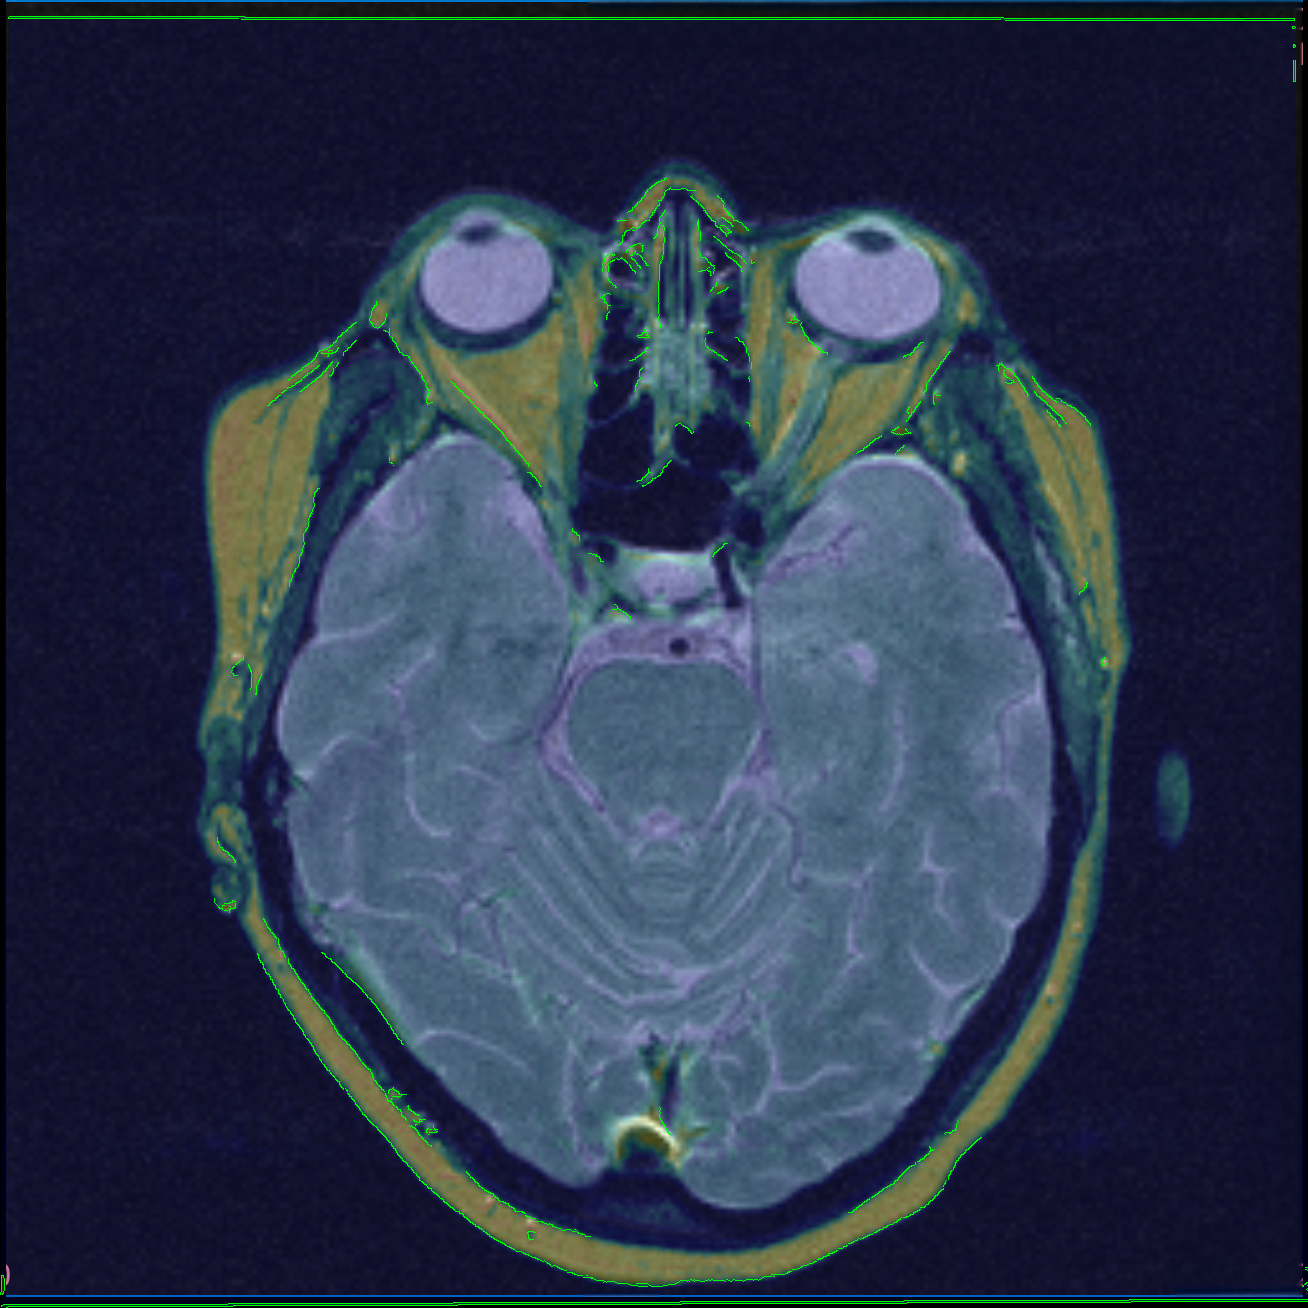
\includegraphics[height=.13\textheight]{./figure/compare_opencv_3.png}
			\caption{图像配准效果示意3}
		\end{subfigure}
		
		\caption{基于SIFT算法及RANSAC算法的图像配准}
	\end{figure}
	
	基于上述实验分析,我们可以得出结论,传统的端对端配准方案虽然能够在某些局部区域实现较高精度的配准,但在处理复杂医学图像(特别是跨模态配准任务)时仍然存在较大的改进空间。特别是在关键点提取与匹配阶段,传统方法的表现受限于图像模态差异与组织结构特性,难以保证足够的关键点匹配数量。因此,未来的研究可以探索更加鲁棒的特征提取方法,例如结合基于学习的方法,通过深度学习网络提取跨模态鲁棒特征,从而提高匹配稳定性。此外,强化学习方法也可以用于优化配准过程,使得配准变换矩阵的估计更加精确,从而提升整体的配准质量 \cite{reg}。
	
	\section{结论}
	
	本次作业基于 Harris 角点检测、HOG 和 SIFT 特征提取方法,并结合 RANSAC 进行误匹配剔除,成功实现了高精度的全景图拼接。实验结果表明,这种方法能够有效检测和匹配图像中的关键特征点,并利用稳健的变换估计算法,使得拼接结果在视觉上具有较高的连续性和一致性。
	
	在实验中,Harris 角点检测在特征点提取方面表现稳定,能够准确定位图像中的关键点。然而,其对尺度变化的适应性有限,因此结合了 HOG 和 SIFT 特征,以增强特征匹配的稳健性。HOG 特征对光照变化的鲁棒性较强,而 SIFT 具有良好的尺度和旋转不变性,在不同拍摄角度下依然能提供可靠的匹配点。RANSAC 算法在误匹配剔除方面起到了关键作用,通过随机采样和一致性评估,有效减少了错误匹配点的干扰,提高了变换矩阵的精度,从而保证了最终拼接结果的质量。
	
	尽管本次实验在全景图拼接方面取得了良好的效果,但仍存在一定的优化空间。首先,在特征匹配过程中,SIFT 计算复杂度较高,在大规模数据集或实时应用中可能成为瓶颈。因此,未来可以探索加速 SIFT 计算的方法,例如采用 KD-Tree 进行高效近邻搜索或引入深度学习方法进行特征提取。其次,虽然 RANSAC 能够有效剔除误匹配点,但其随机性导致计算效率受采样次数影响较大,可以考虑使用优化的 RANSAC 变种,如 PROSAC 或 LMEDS,以提高收敛速度和匹配精度。此外,当前的拼接方法主要依赖于仿射变换矩阵,对于具有更复杂几何形变的场景,例如非刚性变形或视差较大的图像,可能无法得到理想的拼接效果。未来可结合深度学习的非刚性配准技术或优化配准损失函数,以提升拼接的适用性。
	
	\let\cleardoublepage\clearpage
	
	\begin{thebibliography}{99}
		\bibitem{derpanis_ransac} Derpanis K G. Overview of the RANSAC Algorithm[J]. Image Rochester NY, 2010, 4(1): 2-3.
		\bibitem{derpanis_harris} Derpanis K G. The harris corner detector[J]. York University, 2004, 2(1): 2.
		\bibitem{dip} Gonzales R C, Woods R E. 数字图像处理[M]. 阮秋琦, 阮宇智\ 译. 第4版. 北京:电子工业出版社, 2020 :584-648.
		\bibitem{reg} Hu J, Luo Z, Wang X, et al. End-to-end multimodal image registration via reinforcement learning[J]. Medical image analysis, 2021, 68: 101878.
		\bibitem{hu_hog} Hu R, Collomosse J. A performance evaluation of gradient field hog descriptor for sketch based image retrieval[J]. Computer Vision and Image Understanding, 2013, 117(7): 790-806.
		\bibitem{rire} Kitware. The Retrospective Image Registration Evaluation Project[EB/OL]. 2021[2025-03-29]. https://rire.insight-journal.org/.
		\bibitem{kok_harris} Kok K Y, Rajendran P. Validation of Harris detector and eigen features detector[C]//IOP Conference Series: Materials Science and Engineering. IOP Publishing, 2018, 370(1): 012013.
		\bibitem{mortensen_sift} Mortensen E N, Deng H, Shapiro L. A SIFT descriptor with global context[C]//2005 IEEE Computer Society Conference on Computer Vision and Pattern Recognition (CVPR'05). IEEE, 2005, 1: 184-190.
		\bibitem{siftransac} Shi G, Xu X, Dai Y. SIFT feature point matching based on improved RANSAC algorithm[C]//2013 5th International Conference on Intelligent Human-Machine Systems and Cybernetics. IEEE, 2013, 1: 474-477.
		\bibitem{tatu_hog} Tatu A, Lauze F, Nielsen M, et al. Exploring the representation capabilities of the HOG descriptor[C]//2011 IEEE international conference on computer vision workshops (ICCV Workshops). IEEE, 2011: 1410-1417.
		\bibitem{wu_sift} Wu J, Cui Z, Sheng V S, et al. A Comparative Study of SIFT and its Variants[J]. Measurement science review, 2013, 13(3): 122.
		\bibitem{yaniv_ransac} Yaniv Z. Random sample consensus (RANSAC) algorithm, a generic implementation[J]. Imaging, 2010.
	\end{thebibliography}
	
\end{document}